% !TEX output_directory = ./build

\documentclass[master,english]{hgbthesis}
% Zulässige Class Options:
%   Typ der Arbeit: diplom, master (default), bachelor, praktikum
%   Hauptsprache: german (default), english
%%------------------------------------------------------------

\graphicspath{{images/}}    % wo liegen die Bilder?
\bibliography{library}  	% Angabe der BibTeX-Datei, % utf8-change

\usepackage{tikz}
\usepackage{subfigure}
\usepackage{pgfplots}
\usepackage{amsmath}
\usepackage{amsmath,amssymb}
\usepackage{mathtools}
\usepackage{hyperref}
\usepackage{float}
\usepackage[algo2e]{algorithm2e}
\usepackage[top=3cm,left=3cm,right=3cm,bottom=3cm]{geometry}
% Scriptsize axis style.
\usepackage{bookmark}
\pgfplotsset{every axis/.append style={tick label style={/pgf/number format/fixed},font=\scriptsize,ylabel near ticks,xlabel near ticks,grid=major}}

\usetikzlibrary{shapes.geometric,shapes.arrows,decorations.pathmorphing}
\usetikzlibrary{matrix,chains,scopes,positioning,arrows,fit}


\DeclareMathOperator*{\argmin}{argmin}
\DeclareMathOperator{\E}{\mathbb{E}}
\DeclareMathOperator{\set}{\Bbb{E}}
\DeclarePairedDelimiter{\ceil}{\lceil}{\rceil}

%%%----------------------------------------------------------
\begin{document}
%%%----------------------------------------------------------

% Einträge für ALLE Arbeiten: --------------------------------
\title{Solving localization problem in first person computer games with deep learning}
\author{Yauheni\ Selivonchyk}
\studiengang{Computer Science}
\studienort{Rheinische Friedrich-Wilhelms-Universität Bonn}
\abgabedatum{2017}{03}{30}	% {YYYY}{MM}{DD}

%%% zusätzlich für eine Bachelorarbeit: ---------------------
\nummer{2787799}   % XX...X = Stud-ID, z.B. 0310238045-A
                        % (A = 1. Bachelorarbeit)
\semester{Sommersemester 2017}
\gegenstand{Einführung in die Tiefere Problematik 1}
\betreuer{Prof. Dr. Christian Bauckhage} % oder \betreuerin{..}

%%% zusätzlich für einen Praktikumsbericht: -----------------
\nummer{XXXXXXXXXX-B}   % XX...X = Stud-ID, z.B. 0310238045-B
                        % (B = 2. Bachelorarbeit)
\betreuer{Mag.~Pjotr I.~Czar\\Creative Director}  % \betreuerin{..}
\firma{%
   Oligarchic Media International GmbH\\
   Online Division\\
   1020 Wien, Hubertusgasse 3a
}
\firmenTel{1-234-5678-100}
\firmenUrl{www.mogul.at}

%\strictlicense  % erzeugt restriktive Lizenzformel

%%%----------------------------------------------------------
\frontmatter
\maketitle
\tableofcontents
%%%----------------------------------------------------------

% \include{vorwort}		% ggfs. weglassen
% \include{kurzfassung}
% !TEX root = ./thesis.tex

\chapter{Abstract}

\begin{english}

Localization problem is an important task in Artificial Intelligence (AI).
Extracting and maintaining high accuracy spatial information is crucial for most artificial actors, as automated robots, self-driving vehicles or AI characters in a computer game.
In this work we propose a method, for extracting spatial information from unlabeled continuous visual data using a regularized deep learning model.
We justify existence of a low-dimensional topological space in which actor's movements create a dense trajectory.
Then we propose a technique, that extracts a lower-dimensional encoding of visual data while simultaneously  tries to preserve spatial relations in the encoding space.
We analyze effectiveness of the proposed technique using data, collected with a 3D engine of a first-person shooter game \texttt{Doom II}.

\end{english}


%%%----------------------------------------------------------
\mainmatter         % Hauptteil (ab hier arab. Seitenzahlen)
%%%----------------------------------------------------------

% !TEX root = ./thesis.tex

\chapter{Introduction}
\label{ch:intro}

% Outline:
% - successes of Neural network models
% - specifically for spacial related field (spatial transformer network, video thing)
% - VizDoom and
% - we propose
% - potential usages of the proposed system: SLAM, loop closure detection
% - analyses description
%
% Space-time video completion \cite{Wexler2004}
% % Deep learning for visual understanding: A review \cite{Guo2016}
%
% Loop closure detection for visual SLAM systems using deep neural networks \cite{Gao2015}
% Authors build a denoising autoencoder with sparse objective adding continuity objective.
% Continuity objective enforces L2 similarity between extracted features for consecutive frames. They use dataset: freiburg2 slam.
%
% Loop Closure Detection for Visual SLAM Using PCANet Features.
% Unsupervised learning to detect loops using deep neural networks for visual SLAM system.
% VLAD-Based Loop Closure Detection For Monocular SLAM \cite{Xia2016, Gao2015a, Huang2016}

Localization tasks represent a significant challenge in artificial intelligence (AI).
In particular, successful localization is extremely important to such AI areas as robotics, self-driving vehicles, and micro-surgery, to name a few \cite{Wang2017, Mountney2006}.
It has many potential applications in simultaneous localization and mapping (SLAM) \cite{Cadena2015, Zikos2016}, loop closure detection \cite{Xia2016, Gao2015a, Huang2016}, and correspondence learning \cite{Boscaini2016}.
These tasks are normally trained with labeled data, which is often limited and difficult to collect.
Meanwhile, recent successes in reinforcement learning \cite{Silver, Lample2016} has shown, that given access to powerful models and abundant amount of training data, learning can be done in loosely supervised way.
Important aspect of such training is availability of gaming engines, that can create large amounts of training data on the go.
We are going to take advantage of these developments, by reusing these data generation techniques for learning localization from unlabeled data.

We expect localization task to be possible to learn in an unsupervised manner.
For a given static environment (say, a room or a map of a computer game) we can exactly describe the view of an actor (player, person) by its current position and the direction of the view.
This allows us to state, that every single image observed by the actor can be unambiguous encoded by a small set of latent variables.
Furthermore, from a continuous nature of actors movement we can expect these variables to form a dense continuous manifold in some space of latent variables.
Given that such a manifold exists, we try to construct it in an unsupervised way with a deep neural network model.

Several models has been successfully applied to unlabeled data allowing to construct a dense manifold representation of some visual concepts \cite{Li2015, Kingma2013, Goodfellow2014}.
While these techniques succeeded in encoding data in a lower dimensional space of independent features, they make no assumption about the nature of these features.
We expect, that extremely low-dimensional representation of the spatially related data  would be tightly coupled with that spatial information.
To enforce this expectation we apply additional constrains to our model to enforce extraction of continuous feature.
Existing research on extracting interpretable features suggest, that such extraction is possible, although might have detrimental effect on the performance of the model \cite{Lei2016, Kulkarni2015}.

An ultimate goal of this project can be viewed as a direct and inverse graphics engine in form of an autoencoder.
The goal can be described as achieving an autoencoder objective in form of perfect image reconstruction, while producing a dense continuous spatial manifold in the latent feature space.
Successfully achieving this goal, we will be able to produce players view given the position and vise-versa: determine possible position of the player by the current view.
This model can behave as an ultimate solution for SLAM, correspondence and loop detection problems.
In that particular case the model itself should learn every detail of the static environment being learned.
We understand, that that goal is unlikely to be fully archived, given limited computational resources, discrete nature of actual training data and often non-static characteristics of real-world environments.

Later chapters are organized as follows.
We continue current discussion in chapter \ref{ch:rewo} by describing resent research advances, relevant to the task at hand.
In chapter \ref{ch:tede} we provide technical details of artificial neural network structure, relevant to our task.
Chapter \ref{ch:mode} describes our learning technique and additional model constrains along with underlying motivation.
Finally, in chapter \ref{ch:eval} we explore the advantages of our method on actual data.
Chapter \ref{ch:conc} concludes the results of our research.

% !TEX root = ./thesis.tex

\chapter{Related work}\label{ch:rewo}

In context of our task we would like to pay attention to two subgroups of deep models.
First of all, we are interested in models focusing on producing interpretable results.
Second of all, while learning from unlabeled data, we are interested in unsupervised learning techniques.

Neural network models has proven to be extremely successful in artificial intelligence domains as computer vision \cite{ILSVRC15}, natural language processing \cite{NIPS2013_5021}, semantic parsing \cite{bordes2012}, and many other.
With that success scientific community has shown a large interested in producing interpretable results, that might give an insight into work of such models \cite{Yosinski2015, Mahendran2014, Zeiler2014, Lei2016}.
The reasons for that include pure scientific curiosity, legal reasons, and improving the robustness of neural networks \cite{Goodfellow2015}.

In deep learning domain one of the common ways to produce interpretable results is by applying an additional constrain, enforcing certain form or structure of intermediate network representation  \cite{Jaderberg2015, Lei2016, Kulkarni2015}.
The constrain function can take form of a simple handcrafted regularization, as a sparsity constrain \cite{Ng2011}, as well as be realized by a dedicated complex subnetwork \cite{Lei2016, Li2015}.
For example, Spatial Transformer Networks \cite{Jaderberg2015} use an additional routine in the neural network to extract parameters for best image transformation before feeding it into the discriminative part of the model.
Other group of authors proposed a technique for rationalization of text classification by restricting neural network to build predictions based on a connected peaces of input text \cite{Lei2016}.
Later technique showed to produce human interpretable results at a price of lower classification accuracy.

A large body of research is dedicated to unsupervised learning techniques on visual data.

One popular class of unsupervised learners is a group of energy-based models.
Restricted Boltzmann machines and Deep Boltzmann machines are among the most prominent members of that group \cite{Ackley1985, Salakhutdinov2009}.
Restricted Boltzmann machine is an undirected graphical model based on a bipartite graph structure.
They learn dependency between input distribution and latent distribution in form of intractable partition function.
Such representation is typically hard to use in both learning and evaluation and usually relies on the computationally expensive Monte Carlo Markov Chain method (MCMC).

Recently, more attention has been given to deep neural models based on Autoencoder paradigm.
Autoencoder is an artificial neural network allowing to compress unlabeled data into a lower dimensional space.
Autoencoders learn by simultaneously projecting data into a more compact representation (encoding) and reconstructing original input from the compressed form (decoding).
Several autoencoder models has led to advances in computer vision tasks.
Stacked convolutional autoencoders allow to archive better results on image classification task \cite{Masci2011}.
Stacked denoising autoencoders showed still better results by learning from data altered by random noise  \cite{Vincent2010}.
Stacked What-Where Auto-encoders allowed to apply models of the kind to broader range of training datasets \cite{Zhao2015}.
Yet, one the most fascinating results in resent years has been achieved by generative models based on autoencoder paradigm.

Generative Moment Matching Networks (GMMNs) \cite{Li2015, Ren2016} augment autoencoder architecture with additional projector network for purposes of data generation.
Projector network maps Gaussian noise of the known form into the encoding space of autoencoder in such a way, that the decodings of the that mapping resembles true data distribution.
The learning objective of the projection network is to generate inputs with similar statistics as the training data.
Using this approach it becomes possible to generate new data by a single pass through the trained network, which is advantageous comparing to costly MCMC sampling.
Method uses stochastic gradient descent for training.
GMMNs author claim that this architecture learns latent manifold on which the data has high density and that generative process yields highly realistic images.
Yet, this approach does not attempt to extract interpretable latent features.

Variational Autoencoders (VAE) use autoencoder approach with additional objective, that input distribution in the feature space must explicitly match some target distribution \cite{Kingma2013, Doersch2016}.
Most commonly, an multi-variant isotropic Gaussian is selected as the target probability distribution.
In case of successful learning, sampling from the target distribution should produce latent codes of some realistic inputs, which can be further projected back into input space using decoder network.
This approach allows learning disentangled latent features of the data distribution in form of components of the target distribution space.

Generative adversarial networks (GANs) \cite{Goodfellow2014} use alike approach of sampling data-points, close to original data distribution, by projecting random samples of explicitly defined latent feature space.
Yet, instead of training the decoder (or generator, in that case) network on the original data directly, as autoencoders do, GANs use additional \textit{discriminator} network.
Discriminator defines training objective for the generator.
Discriminator network trains to distinguish artificial examples produced by the generator from samples of true data distribution.
Generator, at the same time, learns to produce examples indistinguishable from the data distribution by trying to maximize discriminator's error on artificial inputs.
This approach allows to reveal interesting latent representations of the data space that were not archived with other types of models.
As a disadvantage, it proved to be hard to learn combined training objective of the ensemble of two networks.
This complicates the training process.
Furthermore, additional tweaks have to be used to enforce variation in the generator's outputs.
Without it generator is prone to \textit{mode collapse}, when generated outputs are hardly distinguishable from each other regardless of the input values.

Away from generative models a few techniques has been developed to extract useful features with autoencoders.
Sparse autoencoders is one of the examples in context of classification task \cite{Ng2011, Makhzani2013, Masci2011}.
Sparse autoencoders impose additional sparsity constrain on the encoding space.
Such a constrain enforces encoder to have low average activation on the output layer, which highly resembles a neural network trained for classification.
Autoencoder trained this way can be used for initialization of a classification network of a similar architecture.

Unsupervised learning of interpretable concepts received little attention in the literature.

Deep convolution inverse graphics networks (DC-IGNs) make an attempt to extract interpretable features out of visual data \cite{Kulkarni2015}.
DC-IGNs are trained to extract representation of the relevant features, such as spatial orientation of an object or position of a light source.
Ideally, this should allow to manipulate values of the learned features for new inputs.
This approach develops on the idea of VAEs by adding a second encoding space, not controlled by variational objective, for interpretable features.
Network is trained on sequences, depicting relevant feature transformation i.e. changing orientation of a single object in horizontal or vertical plane, or the position of the light source.
This process still requires labeled sequences of visual data for learning process.
We find this model the most relevant for our tasks at hand: learning interpretable latent features from unlabeled visual data.

The work on Understanding Visual Concepts with Continuation Learning \cite{Whitney2016} generalizes approach of DC-IGNs for image sequences.
Their approach is based on the idea, that in a sequence of images image $t+1$ can be reconstructed with high quality by decoding latent representation of the image $t$, given some low-dimensional information about transformation between two images.
To achieve that authors train autoencoder using pairs of subsequent images.
Autoencoder is supposed to reconstruct an image, given encoding of a previous image and some sparse vector, representing transformation.
Transformation is extracted with additional \textit{gating} layer, that has access to information about both images.

At last, it worth mentioning recent progress in neuroscience, which is a common source of inspiration when it comes to designing a neural networks.
There are several discovered types of neurons in mammal brain, responsible for the spatial perception.
\textit{Place cells} is one of the most well-studied class of cells responsible for storing information about current location \cite{Fenton2009, Hartley2014}.
A small number of place cells are active at a time, indicating the current location of the mammal
\textit{Head direction cells} is another group of cells, few of which are firing depending on the current direction of the view \cite{Taube1990, Taube1990a}.
The last major group is \textit{grid cells}, that are responsible for tracking the spatial position within an environment in accordance to individual's movements \cite{Moser2008}.
Within a group of grid cells only few neurons are active at a time and typically newly activated neurons are neighbors of the recently active ones, creating a hexagonal grid-like pattern of activations.
Grid cells are considered to be the positional system of a mammal.
Other known groups on neurons include cells, tracking distance to a known object, or cells, tracking the direction of the boundary of the location \cite{Lever2009}.
Discoveries of cells, that constitute to positional system in the brain, has been awarded the 2014 Nobel Prize in Physiology or Medicine.

% !TEX root = ./thesis.tex

\chapter{Technical details}
\label{ch:tede}

This chapter provides technical details relevant to the method proposed in chapter \ref{ch:mode}.
In subsection \ref{ch:nn} we provide an overview of artificial neural networks and related optimization techniques.
Subsection \ref{ch:ae} describes several unsupervised learning techniques for artificial neural networks also known as autoencoders.

\section{Artificial Neural Networks}
\label{ch:nn}
An artificial neural network is a mathematical model inspired by biological brain structure.
A neural network comprises of a set of interacting computational units, called neurons.
In practice, neurons' computation contains a linear transformation of inputs followed by an activation function.
Sigmoid, ReLU and identity functions are among most commonly used activation function.

Neural networks are organized in layers.
A layer can be viewed as a set of neurons that rely on same inputs and have similar behavior i.e. activation function, output size, regularization parameters.
We also distinguish auxiliary layers that perform some transformation of the input data.
Scaling layer, applying nonlinearity function and pooling layer are one of many examples of such layers.

Major neural networks groups are distinguished between each other by structure of connections between neurons.
Feedforward neural networks prohibit cyclic connection and loops in network structure, while Recurrent neural networks have no such restriction.

In subsection \ref{ch:ffnn} we are going to describe basic building blocks of feedforward neural networks.
Subsection \ref{ch:cnn} describes a special case of feedforward neural network with parameter sharing.
Finally, in subsection \ref{ch:opt} we discuss basic concepts of training artificial neural networks.

% \subsection{Artificial Neural Network}
\subsection{Feedforward Neural Networks}
\label{ch:ffnn}

Let's take a look at the simplest case of an artificial neural network: the perceptron.
The single layer perceptron performs a linear transformation of the input values and subsequently applies some activation function $f$:
\begin{equation}\label{eq:per}
  y = f(\sum_{i=1}^N W_ix_i + b) = f(Wx+b)
\end{equation}
where $W$ is a column vector of perceptron parameters and $f$ is an activation function. The structure of the perceptron is depicted in figure \ref{fig:perc}.

% !TEX root = ../thesis.tex

\begin{figure}

\centering
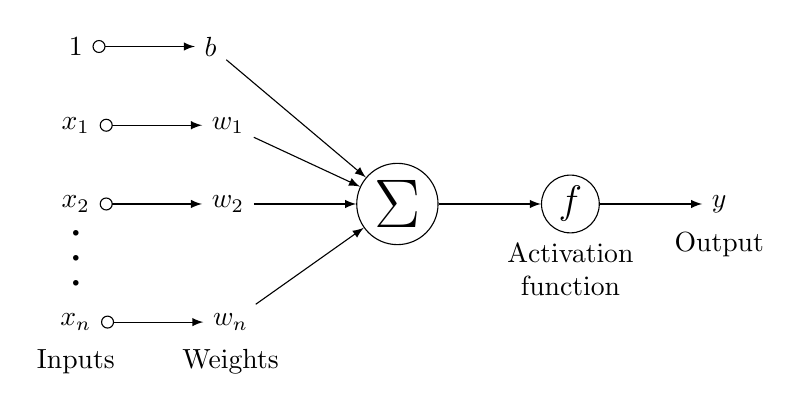
\begin{tikzpicture}
  [
    init/.style={  draw,  circle,  inner sep=2pt,  font=\Huge,  join = by -latex},
    act/.style={  draw,  circle,  inner sep=2pt,  font=\Large,  join = by -latex},
    squa/.style={  draw,  inner sep=2pt,  font=\Large,  join = by -latex},
    start chain=2,node distance=13mm
  ]
  \node[on chain=2] (x2) {$x_2$};
  \node[on chain=2,join=by o-latex] {$w_2$};
  \node[on chain=2,init] (sigma) {$\displaystyle\Sigma$};
  \node[on chain=2,act,label=below:{\parbox{2cm}{\centering Activation \\ function}}] {$f$};
  \node[on chain=2,label=below:Output,join=by -latex] {$y$};
      % {[shift={(0.0,-2.0)}]\centering Activation \\ function}

  \begin{scope}[start chain=4]
  \node[on chain=4] at (0,2.0cm) (b) {$ 1$};
  \node[on chain=4,join=by o-latex] (w0) {$b$};
  \end{scope}

  \begin{scope}[start chain=1]
  \node[on chain=1] at (0,1.0cm) (x1) {$x_1$};
  \node[on chain=1,join=by o-latex] (w1) {$w_1$};
  \end{scope}

  \begin{scope}[start chain=3]
  \node[on chain=3,label=below:Inputs] at (0,-1.5cm) (x3) {$x_n$};
  \node[on chain=3,label=below:Weights,join=by o-latex] (w3) {$w_n$};
  \end{scope}
  % \node[label=above:\parbox{2cm}{\centering Bias \\ $b$}] at (sigma|-w1) (b) {};

  \draw[-latex] (w0) -- (sigma);
  \draw[-latex] (w1) -- (sigma);
  \draw[-latex] (w3) -- (sigma);
  % \draw[o-latex] (b) -- (sigma);

  % \draw[decorate,decoration={brace,mirror}] (x1.north west) -- node[left=10pt] {Inputs} (x3.south west);
  % \draw[decorate,decoration={brace,mirror}] (b.north west) -- node[left=10pt] {Bias} (b.south west);
  \path (x2) -- (x3) node [font=\huge, midway, sloped] {$\dots$};
\end{tikzpicture}
\caption{Structure of a basic computational unit of a neural network (perceptron). Input values $x$ are linearly combined according to the set of parameters $W$ and bias $b$ and activation function $f$ is applied.  }
\label{fig:perc}
\end{figure}


By combining several perceptrons in one set we can produce multiple output values of $y$.
For simplicity, we will stack parameters of $j$ distinct perceptrons that use the same input of size $i$ into matrices $W$ and $b$, where $W$ is rectangular matrix of size $[i,j]$ and $b$ is a column vector of size $j$.
In this case equation $\ref{eq:per}$ remains the same for column vector $y$ of size $j$. A set of perceptron-like neurons that perform computation on the same input forms a single \textit{fully connected} layer of multilayer neural network.

When we combine several layers together we would refer to input vector $x$ as \textit{input layer} and to the last layer of the network producing final output $y$ as \textit{output layer}. All intermediate layers between input and output are called \textit{hidden layers}. We would refer to the depth of the network as to number of computational units on the longest path connecting input and output layers.

It has been shown, that artificial neural network, under mild assumption about the form of the activation function, can act as universal approximator even using a single layer of hidden units of finite size \cite{Debao1993}. Yet, some approximation would require at least exponentially many hidden units in number of inputs $||h||=2^{||x||}$ \cite{Pascanu2014} while using only a single hidden layer. Furthermore, architecutre of $k+1$ layers can be exponentially less complex that architecture of $k$ layers \cite{Bengio2009a}.
Hence, many researchers are developing neural networks with hundreds of layers to allow more compact representations of complex functions \cite{He2015, Srivastava2015}.

Expressivity of the functions that can be approximated by a neural network comes at a cost.
Extensively complex models are prone to overfitting. In other words, models can show excellent performance on the training data while providing poor solutions on yet unseen inputs. In the worst case, an overparameterized model is capable of learning exact mapping between inputs and desired output values without learning useful concepts.

To reduce overfitting several techniques can be used. Reducing model capacity, collecting or generating more training data and regularizing the model are among the most widely used in the context of neural networks.

Using convolutional neural networks is one of the options to reduce capacity of the model by using shared model weights.

Xaviere initializatin \cite{Glorot2010}

% !TEX root = ../thesis.tex

\begin{figure}[t!]
	\centering
	\subfigure[Logistic sigmoid.]{
    		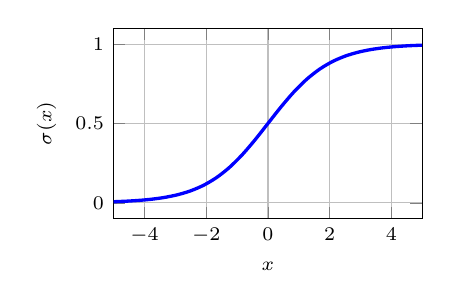
\begin{tikzpicture}
			\begin{axis}[width=5.5cm,height=4cm,ylabel=$\sigma(x)$,xlabel=$x$,ymin=-0.1,ymax=1.1,xmin=-5,xmax=5]
				\addplot[very thick,blue,smooth] {1/(1+exp(-x))};
			\end{axis}
		\end{tikzpicture}
	}
	\subfigure[Hyperbolic tangent.]{
		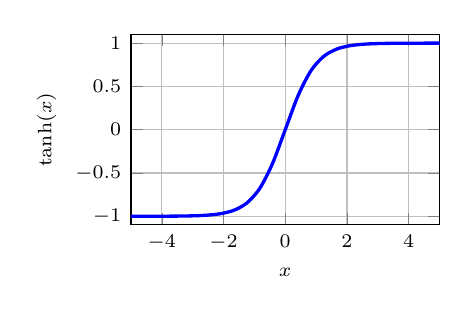
\begin{tikzpicture}
			\begin{axis}[width=5.5cm,height=4cm,ylabel=$\tanh(x)$,xlabel=$x$,ymin=-1.1,ymax=1.1,xmin=-5,xmax=5]
				\addplot[very thick,blue,smooth] {tanh(x)};
			\end{axis}
		\end{tikzpicture}
	}\\
	\subfigure[Rectifier linear unit \cite{Nair2010}.]{
    		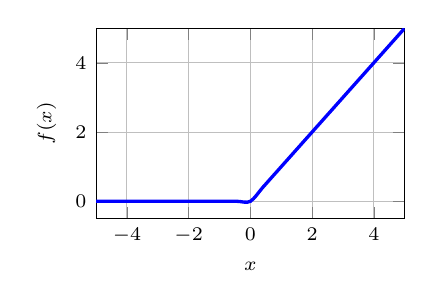
\begin{tikzpicture}
			\begin{axis}[width=5.5cm,height=4cm,ylabel=$f(x)$,xlabel=$x$,ymin=-0.5,ymax=5,xmin=-5,xmax=5]
				\addplot[very thick,blue,smooth] {max(0, x)};
			\end{axis}
		\end{tikzpicture}
	}
	\subfigure[Identity function.]{
		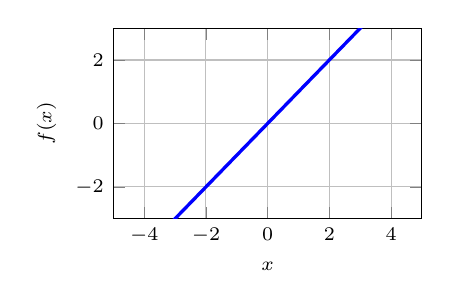
\begin{tikzpicture}
			\begin{axis}[width=5.5cm,height=4cm,ylabel=$f(x)$,xlabel=$x$,ymin=-3,ymax=3,xmin=-5,xmax=5]
				\addplot[very thick,blue,smooth] {x};
			\end{axis}
		\end{tikzpicture}
	}
    	\caption[Sigmoidal activation functions.]{Common choise of activation functions includes logistic sigmoid $\sigma(z)$ and hyperbolic tangent $tanh(z)$. Convolutional neural networks often rely on ReLU and identity functions.}
    	\label{fig:act}
\end{figure}


% \subsection{Artificial Neural Network}
\subsection{Convolutional Neural Networks}
\label{ch:cnn}

The convolutional neural network is a special kind of feedforward neural network that takes advantage of structural organization of the data. This technique allows to decrease the number of parameters of the model when applied to structured data.

Many types of data contain redundant information .i.e. information that, when ignored, can be recovered from the remaining data.
For instance, we can rather easily reconstruct the skipped word in the sentence "\textit{Clouds are in the \_\_}" as well as we can recognize an object on an image when some pixels are altered or missing.
In other words, components of textual or visual data are often interdependent and contain duplicated information.

Convolutional neural networks use small specially adjacent parts of data as neuron inputs. Multiple neurons reuse the same set of parameters $K$, called \textit{kernel}, on distinct patches of the input. All convolutional neurons depending on the same kernel $K$ form a \textit{convolutional filter}. A set of outputs produced by a single convolutional filter is called a \textit{feature map}.



For a 3-dimensional image $I$ of size $H \times W \times C$, where $H$,$W$,$C$ are height, width and number of color channels correspondingly, applying 2-dimensional convolutional filter $K$ of size $w \times h$ would result in a feature map of size $(H-h+1) \times (W-w+1) \times 1$. Kernel $K$ would use $w \times h \times C$ parameters. Convolution operation can be described as:
\begin{equation}\label{eq:conv}
  (I \cdot K)_{x, y} = \sum_a \sum_b \sum_c K_{a,b,c} I_{x+a, y+b,c}
\end{equation}
where ${x, y}$ and ${a,b}$ are two-dimensional indices of feature map and convolution correspondingly and follow next constrains:
\begin{equation*}
  \begin{aligned}
  &1 \leq  x \leq H-h+1, \\
  &1 \leq  y \leq W-w+1, \\
  &1 \leq  a \leq h, \\
  &1 \leq  b \leq w, \\
  &1 \leq  c \leq C.
\end{aligned}
\end{equation*}

\begin{figure}
  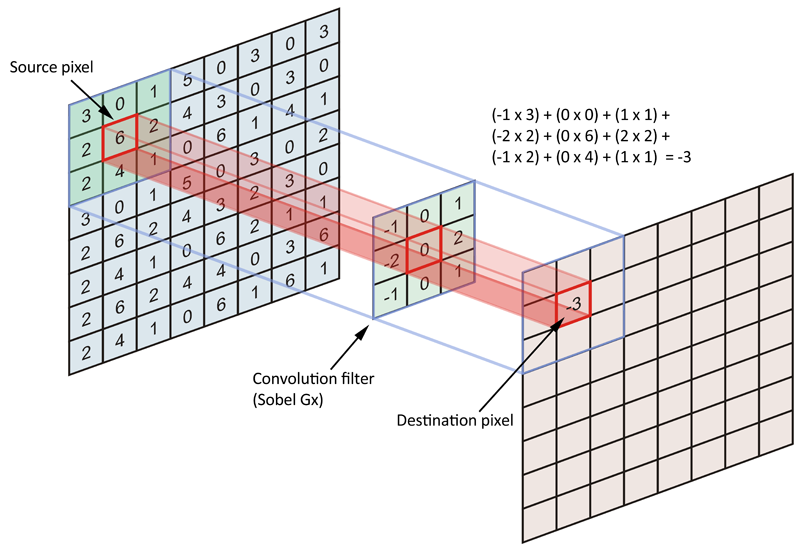
\includegraphics[width=\textwidth,height=\textheight,keepaspectratio]{cnn.png}
  \caption{Illustration of applying convolutional filter of size 3x3 to a single square patch. Output feature map is padded to preserve same shape as input data. Picture taken from [community.arm.com]}
  \label{fig:cnn}
\end{figure}

To preserve width and hight of the feature map $(I \cdot K)$ equivalent to the source image we can add padding along the edges of the input. We can duplicate the same values or use zeros as a padding.
Further, we can apply $k$ distinct convolutional filters to produce output volume of size $x \times y \times k$.

Output of convolution \ref{eq:conv} is often summed with an additional bias $b$ before further processing.
The bias is shared across all convolutional neurons depending on the same kernel.
Value $(I \cdot K)_{x, y}+b$, called \texttt{preactivation}, is forwarded to activation function $\sigma$.

The activation operation can be followed by a pooling operation.
Pooling replaces the output of the convolution layer with summary statistics of nearby outputs.
Max-pooling is one example of such an operation.

\subsubsection{Max-pooling layer}

Max-pooling is a pooling operation applied independently to every feature map.
Max-pooling replaces the output of $\sigma((I \cdot K)_{x, y}+b)$ with a maximum value over a small region of size $w$, $h$ centered at point $(x,y)$.

We can use convolutional and pooling operations in \texttt{strided} mode. When using strides instead of applying operation to every unique position $(x, y)$ we can skip over some indices. Applying strides greater than $1 \times 1$ results in decrease in size of the feature map. For an image of size $H \times W \times C$ and max-pooling operation with stride $h \times w$ we can calculate size of the output feature map as follows $H_o \times W_o \times C $:
\begin{equation*}
  \begin{aligned}
  & W_o = \ceil[\bigg]{\frac{W}{w}} \\
  & H_o = \ceil[\bigg]{\frac{H}{h}} \\
\end{aligned}
\end{equation*}

Downsampling is essential to reduce computational complexity of the network.
Downsampling with pooling layers improves positional tolerance of convolutional networks.
Strided pooling is preferred to strided convolution operation for downsampling. Strided pooling layers are shown to work better in practice, allegedly, due to greater amount of valuable information preserved after downsampling.

Max-pooling operation does not rely on any internal parameters. During training, the position of the maximum element has to be stored. During backpropagation gradients are applied only to the position of the maximum value. Non-maximum elements of the input feature map do not contribute to the total error since they are not used by the upper layers of the network.

\subsection{Network parameters learning}
\label{ch:opt}

TODO: rework with empirical risk minimization in mind. introduce notion of generalization error

Even though a multilayer neural network can approximate large family of compact functions arbitrary well \cite{Debao1993}, finding the right parameters for such approximation is non-trivial.
Lets consider some error function $L(y, f(x, \theta))$ that calculates error between expected values $y$ and the output of the function $f$, realized by a neural network depending on parameters $\theta$. Finding the solution for a general neural network is equivalent to solving next optimization problem:

\begin{equation}\label{eq:optnn}
  \hat{\theta} = \argmin_{\theta \in \Bbb{R}^D} J(\theta) = \argmin_{\theta \in \Bbb{R}^D} \frac{1}{N} \sum_{i=1}^{N} L(y_i, f(x_i, \theta))
\end{equation}
where $D$ is equivalent to number of parameters $||\theta||$ and $N$ is the size of the training set.

Problem \ref{eq:optnn} has no closed-form solution and finding optimal set of parameters $\hat{\theta}$ is an NP-hard problem \cite{Anandkumar16}.
In practice, gradient descent methods are used to find good parametrization $\hat{\theta}$ of the neural network.

Gradient descent methods suggests to iteratively update parameters $\theta_t$ each time taking a step $\eta$ towards the direction of a better solution $\theta_{t+1}=\theta_t - \eta \nabla_\theta \theta$ \cite{Cauchy1847}.
We use vector partial derivatives $\nabla_\theta J(\theta)=\{ \frac{\partial J(\theta)}{\partial w_1}, \ldots, \frac{\partial J(\theta)}{\partial w_N} \}$ of function $J(\theta)$ at point $\theta_t$ as the the direction towards a better solution. Gradient descent method requires both functions $L(y, \hat{y})$ and $f(x, \theta)$ to be differentiable. Note, that differentiability of function $f(x, \theta)$ in $\theta$ implies differentiability of the activation function \ref{eq:per}. Algorithm pseudocode is shown on listing \ref{alg:bp}.

% !TEX root = ../thesis.tex

\begin{algorithm}[H]
 \KwData{X, Y  \text{ (Train set)}}
 \KwResult{$\theta \text{ (Learned weights)}$}

 ${\textbf{Require: } \eta\text{: Stepsize}}$

 $\theta \gets \theta_0 \text{ (Initialization)}$

 \While{not time to terminate}{
  $\triangle_\theta \gets \nabla_\theta J(\theta)(X, Y) \text{ (Calculate gradients)}$

  $\theta \gets \theta - \eta \triangle_\theta\text{ (Update weights)}$

 }

 \Return $\theta$

 \caption{Gradient descent algorithm}\label{alg:bp}

\end{algorithm}


Gradient based methods do not guarantee to find the optimal solution.
Traing can stop in a local minima ($\theta \leq \theta + \eta \delta | \forall \delta \text{ s.t. } |\delta|^2 \leq \epsilon$) or a saddle point.
These cases are shown on figure \ref{fig:critical}.

\begin{figure}[h!]
  \centering
    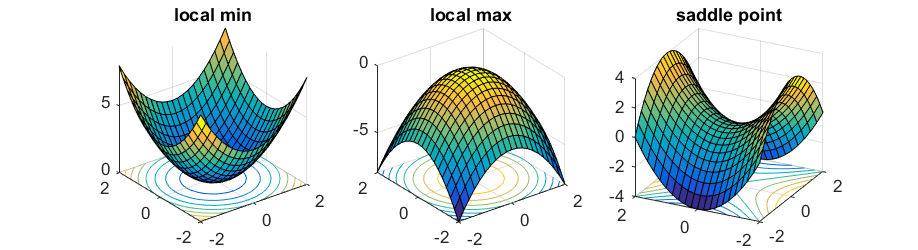
\includegraphics[width=\textwidth,height=\textheight,keepaspectratio]{minmaxsaddle.png}
  \caption{Critical points of a loss function $f(x)$, where $x \in \Bbb{R}^2$.}
  \label{fig:critical}
\end{figure}

In practice, solutions produced by gradient based methods have proven to have satisfying qualities \cite{Szegedy2016,He2015}.
This might be due to the properties of high-dimensional non-convex error surfaces. The study by Y.Dauphin et al. \cite{Dauphin14} concludes, that saddle points and local minima on such surfaces are very likely to be close to global minima.

\subsubsection{Stochastic gradient descent with mini-batches}

Algorithm \ref{alg:bp} requires full path through the complete training set on each iteration.
This might be computationally wasteful for large datasets. Instead, we can perform optimization iteratively only considering subsets of the training set, drawn i.d.d. from the training set:

\begin{equation*}\label{eq:sopt}
  \begin{aligned}
  & \frac{1}{N} \sum_{i=1}^{N} L(y_i, f(x_i, \theta)) = \E_{i \sim U(1,N) } L(y_i, f(x_i, \theta)) \\
  & \E_{i \sim U(1,N) } L(y_i, f(x_i, \theta))= \frac{1}{M} \E_{m \sim U^M(1,N) } \sum_{i \in m} L(y_i, f(x_i, \theta))
  \end{aligned}
\end{equation*}

As a result, we can use the stochastic procedure of selecting $M$ inputs from the training dataset to use in each training iteration.
Subset of inputs selected this way are called \textbf{mini-batches}. Updated algorithm is shown on listing \ref{alg:sbp}.

% !TEX root = ../thesis.tex

\begin{algorithm}[H]
 \KwData{X, Y  \text{ (Train set)}}
 \KwResult{$\theta \text{ (Learned weights)}$}

 $\textbf{Require: } \eta\text{: Stepsize}$

 $\textbf{Require: } M \text{: Minibatch size}$

 $\theta \gets \theta_0 \text{ (Initialization)}$

 \While{not time to terminate}{
  $X_i, Y_i \gets \text{Select $M$ examples i.i.d. from $X, Y$}$

  $\triangle_\theta \gets \nabla_\theta J(\theta)(X_i, Y_i) \text{ (Calculate gradients)}$

  $\theta \gets \theta - \eta \triangle_\theta\text{ (Update weights)}$

 }

 \Return $\theta$

 \caption{Stochastic gradient descent algorithm with minibatches}\label{alg:sbp}

\end{algorithm}


\subsubsection{Backpropagation algorithm}

\subsubsection{Adam update rule}

Training time of gradient descent based algorithm can be reduced by applying adaptive learning rates \cite{Kingma2015}.
\textit{Adam update rule} or simply Adam is one of the algorithms that allow to reduce training time of gradient descent.

The Adam update rule maintains exponential moving average of the gradients $m_t$ and the squared gradient $v_t$.
Hyperparameters $\beta_1, \beta_2$ set the exponential decay rates for both sets of variables.
The update rule for exponential moving average is as follows:
\begin{equation*}
  \begin{aligned}
    & m_t = \beta_1 \cdot m_{t-1} + (1-\beta_1) \cdot g_t \\
    & v_t = \beta_2 \cdot v_{t-1} + (1-\beta_2) \cdot g_t^2
  \end{aligned}
\end{equation*}

Variables $m_t$ and $v_t$ are estimating 1st and 2nd moments of the gradients.
We can therefore rewrite update rule:
\begin{equation}
  \theta_t \gets \theta_{t-1} - \frac{\eta m_t}{\sqrt{v_t} + \epsilon}
\end{equation}
where $\epsilon$ is a small guard value that prevents the divisor from getting too close to zero.

Exponential moving averages $m_t$ and $v_t$ are initialized with zeros.
This leads to zero-bias of the estimators during initial phase of the training.
To accelerate the learning process during first iterations of algorithm \ref{alg:sbp} a time dependent regularization is applied:
\begin{equation*}
  \begin{aligned}
    & \hat{m} = m / (1-\beta_1^t) \\
    & \hat{v} = v/(1-\beta_2^t)
  \end{aligned}
\end{equation*}
where $t$ is a variable tracking current iteration number.

The algorithm requires memory overhead proportional to the number of parameters $||\theta||$. Listing \ref{alg:adam} shows the full algorithm of Adam update rule written in pseudocode.

% !TEX root = ../thesis.tex

\begin{algorithm}[H]
	\KwData{X, Y  \text{ (Train set)}}
	\KwResult{$\theta \text{ (Learned weights)}$}

	$\textbf{Require: } \eta\text{: Stepsize}$

	$\textbf{Require: } \beta_1, \beta_2 \in [0, 1) \text{: Exponential decay rates for the moment estimates}$

	$\textbf{Require: } f(\theta) \text{: Stochastic objective function with parameters } \theta$

	$\textbf{Require: } \theta_0 \text{: Initial parameter vector}$

	$m_0 \gets 0 \text{ (Initialize 1st moment vector)}$

	$v_0 \gets 0 \text{ (Initialize 2nd moment vector)}$

	$t \gets 0 \text{ (Initialize timestep)}$

	\While {$\theta_t$ not converged}{

		$t \gets t + 1$

		$g_t \gets \nabla_\theta f_t(\theta_{t-1}) \text{ (Get gradients w.r.t. stochastic objective at timestep t)}$

		$m_t \gets \beta_1 \cdot m_{t-1} + (1-\beta_1) \cdot g_t \text{ (Update biased first moment estimate)}$

		$v_t \gets \beta_2 \cdot v_{t-1} + (1-\beta_2) \cdot g_t^2 \text{ (Update biased second raw moment estimate)}$

		$\hat{m}_t \gets m_t / (1-\beta_1^t) \text{ (Compute bias-corrected first moment estimate)}$

		$\hat{v}_t \gets v_t/(1-\beta_2^t) \text{ (Compute bias-corrected second raw moment estimate)}$

		$\theta_t \gets \theta_{t-1} - \eta \cdot \hat{m}_t / (\sqrt{\hat{v}_t}+\epsilon) \text{ (Update parameters)}$
	}
	$\textbf{return: } \theta_t \text{ (Resulting parameters)}$

	\caption{Adam, stochastic optimization algorithm. Default settings that work good for tested problems $\eta=0.0001 \ldots 0.001$, $\beta_1=0.9$, $\beta_2=0.999$ and $\epsilon=10^{-8}$} \label{alg:adam}

\end{algorithm}


\subsection{Regularization}

\subsubsection{Bagging}
\subsubsection{Dropout}

Applying an ensemble of models guarantees to perform not worse than any of ensemble members but the computational complexity of the training and evaluation grows linearly with the size of the ensemble. This might play a limiting factor on the size of the ensemble, especially when training of even a single model is computationally expensive.

The \textit{dropout} technique allows to approximately achieve ensemble performance at relatively low computational overhead \cite{Srivastava2014}.
The dropout authors propose to ignore a randomly chosen subset of non-output neurons during training. A new subset of units is selected for each mini-batch or even for each training example.

Training a model with dropout resembles training an ensemble of models. The models automatically follow the same layer structure and share neuron parameters. The number of possible models indirectly trained with dropout is roughly exponential in the number of non-output units $2^{||N||}$. Dropout prohibits only model graphs with broken connection between input and output units. Of course, these models are not trained explicitly and only a small subset is used during the training process. For training with dropout we can update optimization problem \ref{eq:optnn} as follows:

\begin{equation}\label{eq:optnndo}
  \hat{\theta} = \argmin_{\theta \in \Bbb{R}^D} \E_\mu J(\theta, \mu) = \argmin_{\theta \in \Bbb{R}^D} \E_\mu \frac{1}{N} \sum_{i=1}^{N} L(y_i, f(x_i, \theta, \mu))
\end{equation}
where $\mu$ is a random mask.

This way during the training process we minimize the value of $\E_\mu J(\theta, \mu)$ iteratively sampling masks $\mu$ and minimizing function $J(\theta, \mu)$ for this masks explicitly.

To perform prediction with such a model we need to collect votes from an exponential number of ensemble members.
In practice the following two methods are commonly used. First, alike during the training process, we can sample some constant number $N$ of masks $\mu$ and use majority vote on a small subset of functions $\{f(x, \theta, \mu_1), \ldots, f(x, \theta, \mu_N)\}$. Alternatively, it has been shown that simply multiplying the weight of the layers by \textit{keep probability} provides a good approximation of stochastic evaluation \cite{Srivastava2014}. Later method requires only a single forward pass through the complete network for each prediction.

At last, dropout becomes especially useful when it is hard to control the actual model complexity. Developing or even fine-tuning a new task specific neural network architecture is a demanding process. It becomes more common to reuse an existing network architecture as Inception or ResNet \cite{He2015, Szegedy2016}. Even though number of parameters in this networks can be overwhelming for a particular task, rigorous regularization with dropout might be sufficient to achieve satisfactory results.


\section{Autoencoders}\label{ch:ae}
An autoencoder or an autoassociator neural network is an unsupervised learning algorithm that sets target output values equal to input values $y_i=x_i$ \cite{Ng2011,RanzatoMarcAurelio2007}.
Autoencoders are usually trained according to the \textit{encoder-decoder} paradigm.
Which first allows to project or encode input $x_i$ into some useful feature representation $h_i$.
Then reconstruct or decode the original input $\hat{y_i}$ from representation $h_i$.
This schematically depicted on figure \ref{fig:ae}.


% !TEX root = ../thesis.tex

% \begin{figure}[h!]
%   % \centering
%     
\includegraphics[width=\textwidth,height=\textheight,keepaspectratio]{ae.png}
%   \caption{Autoencoder.}
%   \label{fig:ae}
% \end{figure}


\begin{figure}

\centering
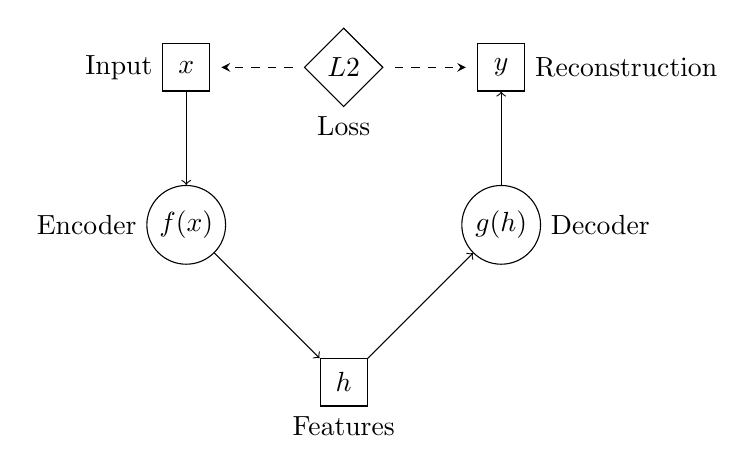
\begin{tikzpicture}
  [
    state/.style={draw, rectangle, minimum width=6mm, minimum height=6mm, inner sep=2pt},
    func/.style={draw, circle, minimum width=1cm, minimum height=1cm, inner sep=2pt},
    loss/.style={draw, diamond, minimum width=1cm, minimum height=1cm, inner sep=2pt},
    node distance=20mm,
    classical/.style={dashed,->,shorten >=4pt,shorten <=4pt,>=stealth}
  ]
  \node (x) [state, label=left:Input] {$x$};
  \node (f) [func, below of=x,label=left:Encoder] {$f(x)$};
  \node(h)[state, below of=f, right of=f,label=below:Features]{$h$};
  \node(g)[func, above of=h, right of=h,label=right:Decoder]{$g(h)$};
  \node(y)[state, above of=g, label=right:Reconstruction]{$y$};
  \node(l)[loss, right of=x, label=below:Loss]{$L2$};

  \draw [->] (x) -- (f);
  \draw [->] (f) -- (h);
  \draw [->] (h) -- (g);
  \draw [->] (g) -- (y);
  \draw [classical] (l) -- (x);
  \draw [classical] (l) -- (y);
\end{tikzpicture}
\caption{An autoencoder with euclidian reconstruction loss.}
\label{fig:ae}
\end{figure}



We are going to refer to encoder as a deterministic differentiable function $f(x, \theta_f)$ that for a given set of parameters $\theta_f$ maps input $x\in \Bbb{R}^d$ into representation $h \in \Bbb{R}^{d'}$.
Likewise, the decoder is a deterministic differentiable function $g(h, \theta_g)$ depending on parameters $\theta_g$, that maps $h\in\Bbb{R}^{d'}$ into $y\in \Bbb{R}^d$. We will further avoid specifying parameters $\theta_f$ and $\theta_g$ for simplicity.
Given a loss function $L$, for a dataset $X=\{x_0, ..., x_i\}$ we can define the learning objective as follows \cite{Good2016}:

\begin{equation}\label{eq:ae}
\min_{\theta_f, \theta_g}\sum\limits_{x_i \in X}{L(x_i, g(f(x))}
\end{equation}

Learning the identity mapping itself is not particularly useful.
Instead we are often interested in reusing only parts of the autoencoder.
For example, parameters of the encoder $\theta_f$ can serve as a good initialization of a discriminative model \cite{Masci2011, Vincent2010, Zhao2015}.
Such initialization results in minor yet coherent improvement of generalization properties of the model.
Variational Autoencoders, on the other hand, reuse decoder as a generator of new training examples \cite{Kingma2013}.
Extracted features $h$ can represent interpretable properties of the input and can be used to adjust this
properties during generation process \cite{Kulkarni2015, Whitney2016}.

Learning useful feature representations is not a trivial task.
One of the common issues with training autoencoders is the possibility to learn an identity mapping of input data.
Learning an identity mapping would result in less informative feature representation of the inputs.
For example, we can represent both encoder and decoder as a linear function and set the size of the feature space so that it exceeds the size of input space $d' > d$.
Then components of autoencoder can both learn simple identity mappings from input space into feature space and vise versa.
Therefore, it is common to either limit the capacity of the feature space to be less than the input space or impose additional regularization on the extracted features.

Additionally, both encoder and decoder can be represented as arbitrary neural networks.
If the capacity of any of the two networks is high enough, it would again lead to learning of an identity mapping.
On the other hand, if the capacity is chosen too low it can hurt the learning process.
For example, low capacity autoencoders are prone to \textit{mode collapse}, when model produces the same output regardless of the input data \cite{Radford2015}.

One of the ways to address the problem of overly high capacity of components can be using stacked autoencoders.
In this approach, instead of directly mapping $h=f(x)$ and $y=g(h)$ into desired lower-dimensional space multiple intermediate mappings can be used $h_i=f_i(h_{i-1})$ and $\hat{h}_i=g_{i+1}(h_{i+1})$.
Stacked autoencoder can be trained in layer-wise manner.
In this case first the mappings $y=g_0(h_0)$ and $h_0=f_0(x)$ are trained.
Then follows training of mappings $y_1=g_1(h_1)$ and $h_1=f_0(h_0)$ and so forth.
The architecture of stacked autoencoder is shown on figure \ref{fig:sae}
% \ref{fig}

% !TEX root = ../thesis.tex

\begin{figure}

\centering
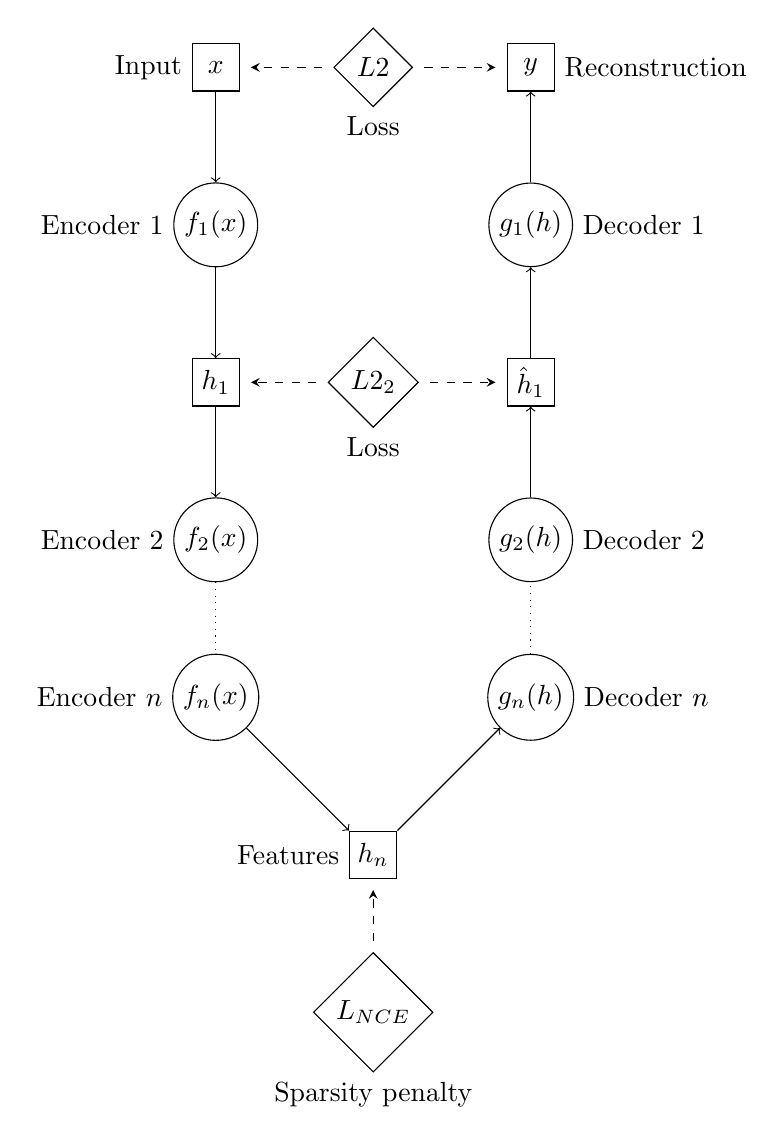
\begin{tikzpicture}
  [
    state/.style={draw, rectangle, minimum width=6mm, minimum height=6mm, inner sep=2pt},
    func/.style={draw, circle, minimum width=1cm, minimum height=1cm, inner sep=2pt},
    loss/.style={draw, diamond, minimum width=1cm, minimum height=1cm, inner sep=2pt},
    node distance=20mm,
    classical/.style={dashed,->,shorten >=4pt,shorten <=4pt,>=stealth},
%     dotted/.style={dotted,-,shorten >=4pt,shorten <=4pt,>=stealth}
  ]
  \node (x) [state, label=left:Input] {$x$};
  \node (f1) [func, below of=x,label=left:Encoder 1] {$f_1(x)$};
  \node(h1)[state, below of=f1]{$h_1$};
  \node (f2) [func, below of=h1,label=left:Encoder 2] {$f_2(x)$};
  \node (fn) [func, below of=f2,label=left:Encoder $n$] {$f_n(x)$};

  \node(hn)[state, below of=fn, right of=fn,label=left:Features]{$h_n$};

  \node(gn)[func, above of=hn, right of=hn,label=right:Decoder $n$]{$g_n(h)$};
  \node(g2)[func, above of=gn, label=right:Decoder 2]{$g_2(h)$};
  \node(y1)[state, above of=g2]{$\hat{h}_1$};
  \node(g1)[func, above of=y1,label=right:Decoder 1]{$g_1(h)$};
  \node(y)[state, above of=g1, label=right:Reconstruction]{$y$};

  \node(l1)[loss, right of=x, label=below:Loss]{$L2$};
  \node(l2)[loss, right of=h1, label=below:Loss]{$L2_2$};
  \node(lnce)[loss, below of=hn, label=below:Sparsity penalty]{$L_{NCE}$};

  \draw [->] (x) -- (f1);
  \draw [->] (f1) -- (h1);
  \draw [->] (h1) -- (f2);
  \draw [dotted] (f2) -- (fn);
  \draw [->] (fn) -- (hn);
  \draw [->] (hn) -- (gn);
  \draw [dotted] (gn) -- (g2);
  \draw [->] (g2) -- (y1);
  \draw [->] (y1) -- (g1);
  \draw [->] (g1) -- (y);

  \draw [classical] (l1) -- (x);
  \draw [classical] (l1) -- (y);

  \draw [classical] (l2) -- (h1);
  \draw [classical] (l2) -- (y1);

  \draw [classical] (lnce) -- (hn);
\end{tikzpicture}
\caption{Stacked autoencoders with euclidian distance as reconstruction loss and negative log-likelihood penalty to enforce sparsity of the extracted features.}
\label{fig:mlae}
\end{figure}



\subsection{Autoencoders in computer vision}\label{ch:dcae}

In this subsection we discuss unsupervised learning techniques specific to vision tasks.
First, we describe the usage of convolutional layers in autoencoders \ref{ch:cae} and data augmentation \ref{ch:denae}.
Subsection \ref{ch:mod_ae} describes possible modifications of learning objective in autoencoders.

Computer vision tasks often have to work with noisy, highly correlated and very high dimensional data. Input size can grow to thousands of features per input example \ref{ILSVRC15}.
Computer vision models have to account for highly nonlinear relation between input features.
Learned concepts have to be highly tolerant to the position of the features on the image grid and be capable to work with spatially transformed and noisy data.
This requirements generally lead to increase in model complexity.

In this subsection we discuss the means of increasing generalization properties of complex computer vision models and modification, more specific to autoencoders.

\subsubsection{Denoising autoencoders}\label{ch:denae}

Learning high capacity models is prone to overfitting.
One of the common ways to decrease overfitting and make model learn useful features without actually changing the model is learning on a larger training corpus.

Denoising autoencoders \ref{Vincent2010} allow to increase variation in training data by adding random noise to images. We construct input examples by adding random noise to the dataset according to some parameter $alpha$: $\hat{x}=n(x, \alpha)$.
Denoising autoencoders are yet supposed to reconstruct  the original image $L(x, g(f(x)))$.
This approach expects encoded representation to be stable and robust under condition of input corruption.
It also expects that the denoising tasks would result in learning useful structure of the input distribution.
Denoising autoencoders are reported to allow better generalization, when an encoded network is used as initializer for the classifier.

\subsubsection{Convolutional autoencoders}\label{ch:cae}

One of the issues commonly encountered in computer vision tasks is spatial correlation of the data.
Neighboring pixels of a single image are rarely fully independent.
Fully-connected networks are ill-fitted for addressing such local correlations of the data.
Furthermore, high dimensionality of computer vision data results in over-parametrization of such models and leads to overfitting.
Recent trends are clearly skewed towards convolutional models \cite{He2015, Szegedy2016} that are consistently showing the best results in computer vision competitions \cite{ILSVRC15, Zhou2016}.

Convolutional and max pooling layers provide means of dimensionality reduction.
As described in section \ref{ch:cnn}, applying strided convolutions or pooling layers leads to a decrease in resolution of the feature map.
Therefore convolutional and max pooling layers are natural candidates for feature extraction in encoder network.

Convolutional networks depend on a relatively small number of parameters.
This quality is desirable for learning a useful feature mapping since it allows to avoid overfitting and, as a result, learning of an identity mapping by the network.
As described in section \ref{ch:cnn}, number of parameters of convolutional layer depends only on kernel size and depth of the feature map.
The number of parameters required by pooling layers is relatively small if not zero and does not depend on the size of the input.

\subsubsection{Deconvolutional layers and input reconstruction}

While convolutional layers are natural for feature extraction in the encoder, reconstruction of highly dimensional input requires a different technique.
One approach is to use an inverse-like operation to convolution.
Deconvolution layer, also known as transposed convolution, is one possible approach.

Deconvolutional layers \cite{Zeiler2010} take as an input an image $y$ composed of $K_0$ color channels $y_1, ... , y_{K_0}$.
As a result of the deconvolution process we would like to obtain $K_1$ feature maps of the same image.
We can represent each channel $c \in [1, \ldots, K_0]$ as $K_1$ channels convolved with feature maps $f_{k,c}$ \ref{eq:conv}:

\begin{equation}\label{eq:de}
  \sum^{K_1}_{k=1}=z^i_k \cdot f_{k,c} = y^i_{k,c}
\end{equation}

where $\cdot$ is a dot product.

Using this equation we would like to find latent feature maps $f_{k,c}$.
Since equation \ref{eq:de} is under-determined and allows multiple solutions.
Therefore a regularization term $z^i_k$ is added to encourage sparsity of the solutions.
With sparsity term we can express the cost function $C$ for input $y_i$:

\begin{equation}\label{eq:dec}
    C(y_i) = \frac{\lambda}{2} \sum^{K_o}_{c=1} ||\sum^{K_1}_{k=1}{z^i_k \cdot f_{k,c} - y^i_{k,c}}||^2_2 + \sum^{K_1}_{k=1}{|z^i_k|^p}
\end{equation}
where we assume mean square error as a reconstruction cost and $p$ as regularization norm.
Constant $\lambda$ balances contributions of the regularization term to the cost function.

Problem \ref{eq:dec} for simplicity can be decomposed into 2 sequential quadratic problems and solved using the stochastic gradient descent method seamlessly with backpropagation.

\subsubsection{Unpooling layers}

Like with convolutional layers, applying pooling layers results in change of the shape of the feature map.
In this subsection we describe a method that allows to effectively revert max-pooling layer preserving the relative spatial position of extracted features as on original image.

In section \ref{ch:cnn} we described applying max pooling layer with some stride $k$.
Applying these layers allows to reduce the size of the feature map up to $k^2$ times while preserving, arguably, most relevant information about the extracted features.
Max-pooling is crucial to convolutional neural networks for achieving some position tolerance of the extracted features \cite{Jaderberg2015}.

The inverse operation of max-pooling is not well defined, since the maximum value must be placed somewhere inside the original volume of size $k^2$. Naively, we can choose an index of a cell index inside projection volume and put maximum values uniformly into the cells with that index.
This procedure is depicted on figure \ref{fig:pool}.
However, this approach destroys relative positioning of unpooled features.
In other words, pooling allows higher lever features to recognize a face by presence of a nose and a mouth within neighboring smaller regions, naive unpooling might place both these features into the same region on the image.

\begin{figure}[h!]
  \centering
    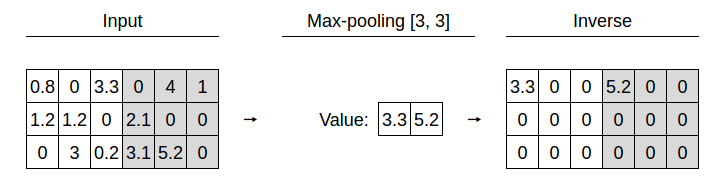
\includegraphics[width=\textwidth,height=\textheight,keepaspectratio]{upsample.png}
  \caption{Upsampling image after max-pooling by placing max value into fixed grid position. Method described by \cite{Dosovitskiy2015a}.}
  \label{fig:pool}
\end{figure}

To address this issue an unpooling layer is introduced. Instead of using information about only the maximum value of the feature in the region, unpooling layers also use information about positioning of the feature. This positional information is called a mask. To every pooled value $x_{i,j}$ corresponds a single mask, indicating the position of the value $x_{i,j}$ inside the pulled volume. We can descripe unpooling operation $up(X, M)$ as follows:

\begin{equation}\label{eq:unp}
  \begin{aligned}
    & Y = up(X, M),\text{ such that} \\
    & \quad X \in \Bbb{R}^{W \times H \times C}, \\
    & \quad Y \in \Bbb{R}^{kW \times kH \times C}, \text{ where $k$ is stride } \\
    & \quad M \in \Bbb{J}^{W \times H \times C}, \text{ where $\Bbb{J}$ is a set of size $|\Bbb{J}|=k^2$ }
  \end{aligned}
\end{equation}

As follows, pooling layers described in section \ref{ch:cnn} must also extract the information $M$ about the positions of maximum values. This modification does not otherwise effect the layer neither during forward nor during backward pass. Application of unpooling layers is illustrated on figure \ref{fig:unpool}.

\begin{figure}[h!]
  \centering
    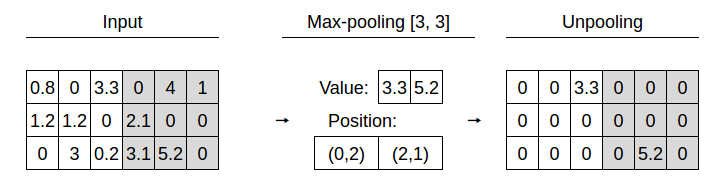
\includegraphics[width=\textwidth,height=\textheight,keepaspectratio]{unpool.png}
  \caption{Illustration of pooling and unpooling layers.}
  \label{fig:unpool}
\end{figure}

Unpooling layers contain no parameters and are not affected by backpropagation.

It's worth noting, that mask information extracted by a modified pooling layer depends on the order of feature channels. As stated by the authors of the original idea, this might have an effect on features, extracted by layers preceding unpooling \cite{Zhao2015}.

\subsubsection{What-Where autoencoders}



\subsection{Extracting useful features with Autoencoders}\label{ch:mod_ae}

The standalone objective \ref{eq:ae} of autoencoders is not particularly useful.
In this section we are going to describe specific use-cases of applying autoencoders along with required modification of objective function.

\subsubsection{Sparse Autoencoders}\label{ch:sae}

Lets consider activations in the hidden layer $h$ for some input $x$:
\begin{equation}
  h(x) = \sigma(W_{h}x_{-1} + b_{h})
\end{equation}
where $W_h$ and $b_h$ are parameters of a hidden layer $h$, $x_{-1}$ is the output of the previous hidden layer and $\sigma$ is some activation function.
Sparse autoencoders introduce an additional term $l_{sparse}$ to the loss function to add a constrain on the activations of the hidden layer $h$ \cite{Ng2011}:
\begin{equation}
  l_{total}(x) = l_{reconstruction}(x, g(f(x))) + \alpha*l_{sparse}(x, h(x))
\end{equation}
where $\alpha$ is a constant parameter.

A sparsity constrain tries to achieve low average activation $\hat{\rho}$ on the hidden layer:

\begin{equation}\label{eq:avgh}
  \rho = \frac{1}{N} \sum_{i=1}^N h_i(x)
\end{equation}

For example, let's take a look at the case for sigmoid activation function in the hidden layer.
Sigmoid produces outputs in the interval $[0, 1]$. If we can guarantee an average activation on the hidden layer $\hat{\rho} \leq 0.1$ we can rely upon the fact that no more than $10\%$ of hidden neurons would have activation close to $1.0$.

A sparse constrain allows to extract useful features even for relatively high number of hidden units. Specifically, a decoder must be able to reconstruct the original representation relying only on few high activation on the hidden layer.

There are several ways to enforce a sparsity constrain.
It is possible to perform gradient descent directly for fixed value of $\hat{\rho}$. In that case we would have to perform a second pass over the dataset to calculate the actual value of $\rho$ to be used as a target during learning with gradient descent. Instead we can simply nullify all but the $k$ highest activation during the forward pass through the network \cite{Kulkarni2015}.
Or apply negative log-likelihood to the hidden layer of the network \cite{Zhao2015}.
At last, to achieve true zero values on the hidden layer we can use an absolute value penalty $l_{sparse}=\sum_{i=1}^N |h_i|$ in conjunction with rectifier a linear unit activation function \cite{Glorot2011}.

Sparse coding of the data has proven to be useful to solve the classification problem.
In particular, the classification task requires us to assign one of $C$ exclusive classes we can train an autoencoder with $C$ hidden units. Once training converges we expect that features, learned by the hidden layer would somewhat correspond to classes of tasks. We can then use the encoder part of the network as initialization of a classifier of the same architecture \cite{Masci2011}.
Such initialization leads to consistently better generalization results after supervised training of the classifier.

\subsubsection{Variational Autoencoders}\label{ch:vae}



% \subsection{Generative adversarial nets}\label{ch:gan}
% \section{Autoencoders and feature interpretability}

% !TEX root = ./thesis.tex

\chapter{Model}

In this chapter we provide overview of our method.
First we provide details about our model initialization and training procedure.
Than we describe baseline architectures that we used as the backbone of our model during evaluation.
At last, we describe our method of robust manifold learning.


\label{ch:mode}

\section{Training process}

In our training we use a server with Intel Xeon CPU 2.40GHz, 64GB of RAM and a GeForce GTX TITAN X Kepler graphics card with 12GB of video memory. Server runs Debian 8.7 operation system with CUDA 8.0, CuDNN 5.1 and TensorFlow 1.0 installed.

\subsection{Tensorflow}

In deep learning TensorFlow \cite{GoogleResearch2015, Abadi2016}, Torch \cite{torch}, and Caffe \cite{jia2014caffe} are among the most common choices of scientific computing framework.
These frameworks use different underlying programming languages and show different compatibility features and qualities of managing computational resources.

We use TensorFlow as our scientific computing framework of choice.

TensorFlow is an open source cross platform software library.
TensorFlow constructs complex computational procedures in form of computational graphs.
Nodes of the computational graph represent some mathematical operations.
Edges of the graph represent data flow between nodes in form of multidimensional arrays, also called tensors.

\begin{figure}[h!]
  \centering
    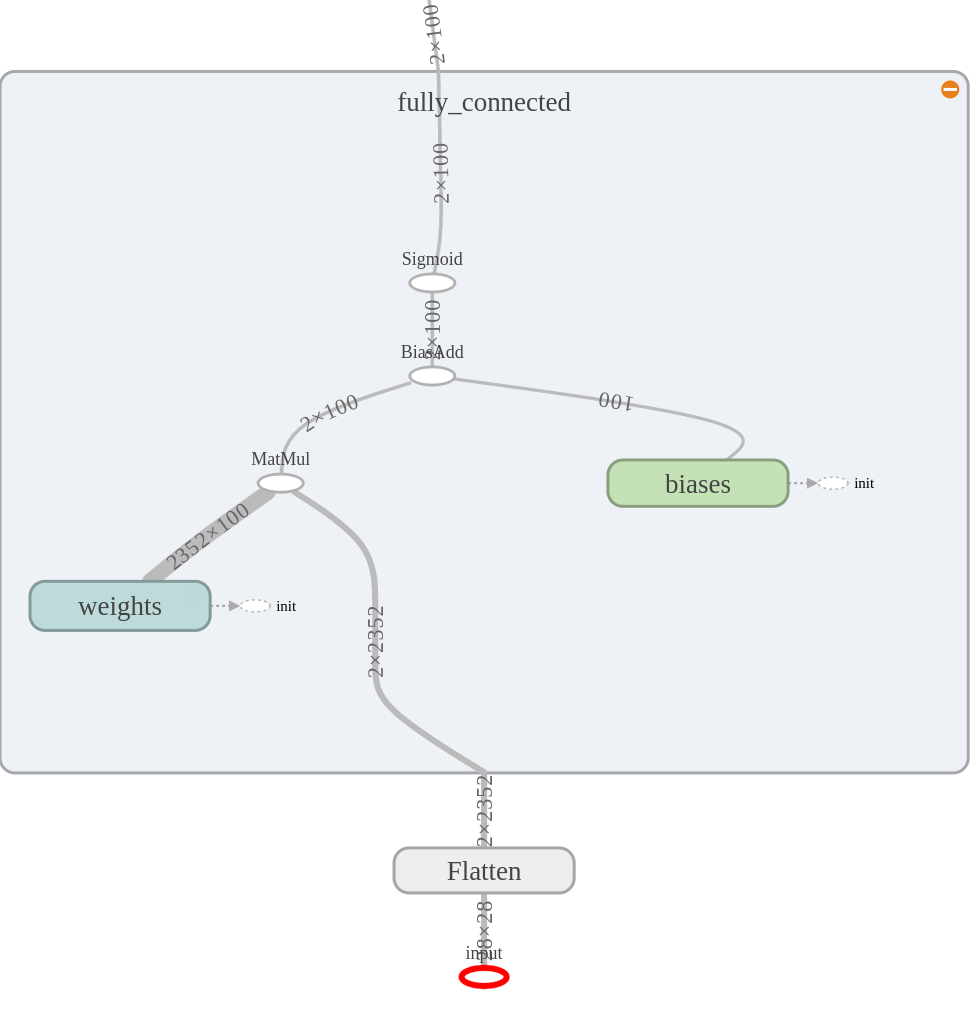
\includegraphics[width=0.7\textwidth,height=0.7\textheight,keepaspectratio]{tf_graph_1.png}
  \caption{TensorFlow detailed graph representation of a single fully connected layer with 100 neurons and sigmoid activation function. Image produced with the build in visualization tool.}
  \label{fig:tf_graph}
\end{figure}

TensorFlow provides cross platform compatibility, which allows to run code on different types of devices and operation systems.
Abstraction over underlying system allows to run models, build with TensorFlow, both on GPUs and CPU without code changes.
Integration with hight performance computing libraries as CUDA \cite{Nickolls2008} and native support of distributed computing makes it a good candidate for computer vision tasks.
An competition winning family of convolutional neural networks Inception is solely developed and maintained on that platform \cite{Szegedy2016}.

We use TensorFlow as our framework of choice for several reasons.
First of all, being a cross-platform frameworks it enables larger audience to reuse results of our research.
Second, it allows to easily configure and run deep network architecture and, at the same time, apply non-trivial modification to the computational flow.
And, at last, it provides build-in visualization tools that allow better control of the learning process.

All our code is shared for public use under MIT License.
\footnote{\url{https://github.com/yselivonchyk/TensorFlow_DCIGN}}

\subsection{Training algorithm}

We run the training using stochastic gradient descent algorithm with mini-batches \ref{alg:bp}. We use adaptive learning rate in form of Adam update rule \ref{alg:adam}. Adaptive learning rate rule has shown to lead to convergence of the backpropagation algorithm at least as often as other methods. It also showed to converge consistently even for a single learning rate for different models.

We use mini-batch size of 128 as the largest one that fits into video memory for each model.
We also found that gradient descent convergence for each of the tested models with learning rate $\nu=0.0001$ is used. This learning rate falls into the interval of recommended learning rates for Adam update rule \cite{Kingma2015}.

We use early stopping as the termination condition of the algorithm \ref{alg:bp}.

To select hyper-parameters of the model, such as weights $\alpha, \beta$ of a composite error $L=L_1 + \alpha L_2 + \beta L_3$, layer sizes etc. we perform a single grid search per parameter.
Grid search is executed for a single parameter at a time, while other parameters stay fixed.
In each grid search is performed for 3 values $\{p_1, p_2, p_3\}$. Whenever better results are achieved for border values $p_1$ or $p_3$, the grid is shifted in the direction of the winning value. When middle value $p_2$ shows the best result but the difference is significant grid search is repeated for decreased grid size.
When parameter shows no effect on model performance the value, that causes better computational efficiency of the model, is selected.

\subsection{Model parameter initialization}

Initial model parameters $\theta$ in conjunction with learning algorithm play crucial role in finding good local minima of optimization problem.
Gradient descent algorithm does not guarantee convergence in finite number of steps.
Hence, model parameters can stay in a "noisy" region where, regardless of learning rate, step in the direction of the gradient on average causes zero decrease of the loss.

It has been shown, that bad weight initialization can lead to exploding or dying out signal especially in deep architectures \cite{Glorot2010}. More specifically, for very small initial weights signal propagating to the further layers becomes too small to be useful and vise versa.
Too large and too small pre-activation values can lead to saturation of sigmoid or tangent units and to dying out of ReLU units. This effectively decreases number of learning units in the network and can impede training.

Most commonly, \textit{Xavier initialization} is used with deep neural networks to avoid situation as described above \cite{Glorot2010}.
Another options might include layer-wise weight initialization, pre-training of the parts of the model \cite{Simonyan2015} or applying weight regularization \cite{Good2016}.
Yet, we would prefer the issue of weight initialization not to effect the training process.


Xavier initializer suggest using normalized initialization, that depends on the number of inputs and outputs of the layer \cite{Good2016}. Weight values are drown uniformly at random from a normal distribution $\Bbb{U}$:

\begin{equation}\label{eq:xavier}
  w_{j, i} \sim \Bbb{U}(
  \mu=-\frac{\sqrt{6}}{\sqrt{n_j+n_{j+1}}},
  \sigma=\frac{\sqrt{6}}{\sqrt{n_j+n_{j+1}}})
\end{equation}

where $i\in\{0, \ldots, |W_j|\}$ is a index of a weight in layer $j$ and $n_j$ is a number of input units of the layer $j$.


\section{Backbone architectures}

In this section we provide overview of three network architectures that we consider useful for trajectory learning from visual data.

All architectures follow multilayer autoencoder design.
Regardless of the backbone, design the last layer of the encoder is a fully connected layer with small (typically smaller than 4) number of computational units.
We would refer to the outputs of this layer as to  \textit{input encoding}.
Additional constrains applied to the encoding are described in section \ref{ss:mf}.

Throughout this work we stick to \textit{mirrored} designed of the encoder and decoder.
This approach allows to have balanced complexity of encoder and decoder subnetworks.

Learning objective of an autoencoder is to reconstruct the original image.
We use $L_2$ $norm$ as the reconstruction loss $L_{reco}$:

\begin{equation}
  L_{2} = \frac{1}{2} \sum_{i, j, c} (x_{i,j,c} - \hat{x}_{i,j,c})^2
\end{equation}

where $x, \hat{x}$ are original image and network output correspondingly.

Input images are encoded in RGBD format. It means that each image pixel $x_{i,j} \in \Bbb{U}^4$ is a 4-dimensional vector.
Each color channel of pixel vector $x_{i,j}$ is a discrete value between 0 and 255: $\Bbb{U} = \{0, 1, \ldots, 255 \}$.
We follow a common practice and treat values discrete values of set $\Bbb{U}$ as continuous values in range $[0.0, 255.0]$.

We scale down input values to allow potential perfect reconstruction by the network.
Scaling is necessary, since activation functions as logistics sigmoid or hyperbolic tangent are upper bounded by 1.0.


\subsection{Fully connected autoencoder}

Fully connected layer of neural networks is a set of computational units, each of which relies on the full set of input parameters of the layer and produces a single output.
We use computational units as described by \ref{eq:per}. We use logistics sigmoid as an activation function.
In this form each fully connected layers with $n_{i-1}$ inputs and $n_i$ outputs rely on $|W_i|=n_{i-1}*(n_i+1)$ parameters.

Work by Jaderberg et al. \cite{Jaderberg2015} suggests, that a fully connected neural network with a single hidden layer might be sufficient to capture spacial information about the input.
In this work, a fully connected \textit{localization net} with a single hidden layer and small number of output units (up to 6) is used to produce transformation parameters for visual data input.
We believe that this architecture represents the most trivial design and use it as a reference backbone model.

Another group of authors successfully applied fully-connected autoencoder to learn latent input representation using Generative Moment-Matching networks \cite{Li2015}. In their experiment, fully connected autoencoders were able to construct dense manifold of the input. For small datasets as MNIST and Toronto Faces Dataset \cite{tfd,lecun-mnisthandwrittendigit-2010} up to 2 hidden layers in both encoder and decoder networks were sufficient.

Fully connected layers rely on huge number of parameters comparing to convolutional and deconvolutional layers.
Number of parameters grows fast with increase in number of layers or number of output units.
This growth of complexity in the parameter space can lead to over-fitting in form of identity learning by the network.

A typical design of an autoencoder network is described by table ?? and depicted on figure ??.
% TODO: add table and figure reference

\subsection{Convolutional autoencoder}

Convolutional models are showing best results in various computer vision competitions in the recent years \cite{ILSVRC15, Zhou2016}.

Convolutional layers of neural networks rely on relatively small number of parameters.
Convolutional neurons typically share the parameters across a single feature map (see section \ref{eq:conv}).

ReLU \cite{Nair2010}



\subsection{WhatWhere autoencoder}

Architecture of What-Where autoencoders \cite{Zhao2015} propose using additional information flow between encode and decoder to improve quality of reconstruction.
What-where autoencoders store the positions of maximum-elements during max-pooling operation to reuse it during reconstruction.
Given positional information decoder no longer have to "guess" the relative position of pooled features during upsampling.

What-where autoencoders in the encoder part use the same architecture as convolutional counterpart.
In the decoder part of the network in addition to transposed convolution \ref{ch:tcnn} an updated upsampling operation is used. Updated upsampling operation called \textit{unpooling} is described in section \ref{ch:unp}.

We consider What-Where autoencoders to be useful for interpretable feature learning, since positional information flow should simplify the process of learning good image reconstruction. This simplification can possibly lead of lesser impact of the noisy $L_{reco}$ error on the learning process.

\begin{figure}[H]
  \centering
  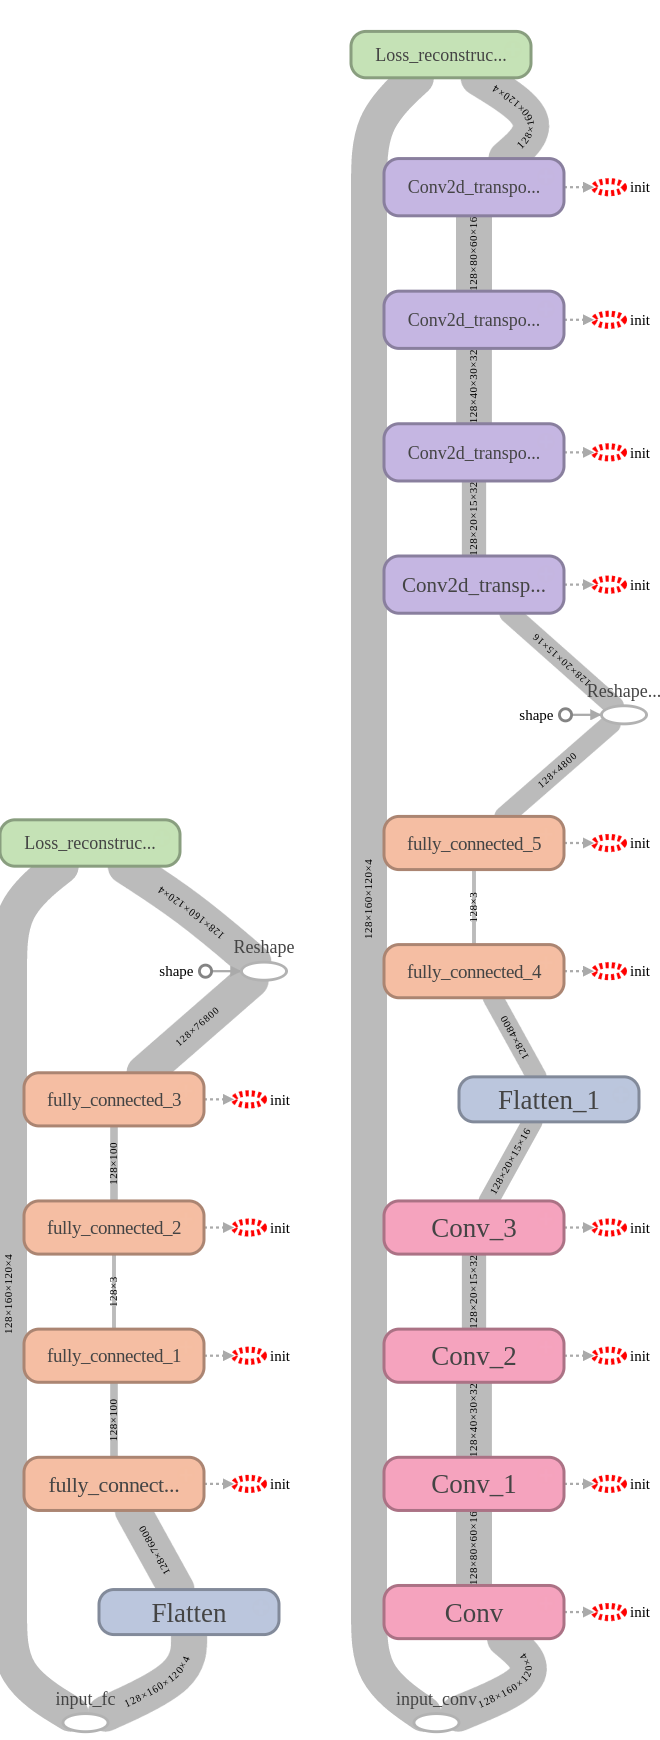
\includegraphics[width=\textwidth,height=\textheight,keepaspectratio]{backbone_1.png}
  \caption{TensorFlow detailed graph representation of a single fully .}
  \label{fig:tf_graph_1}
\end{figure}
% TODO: split into a, b images
\begin{figure}[H]
  \centering
    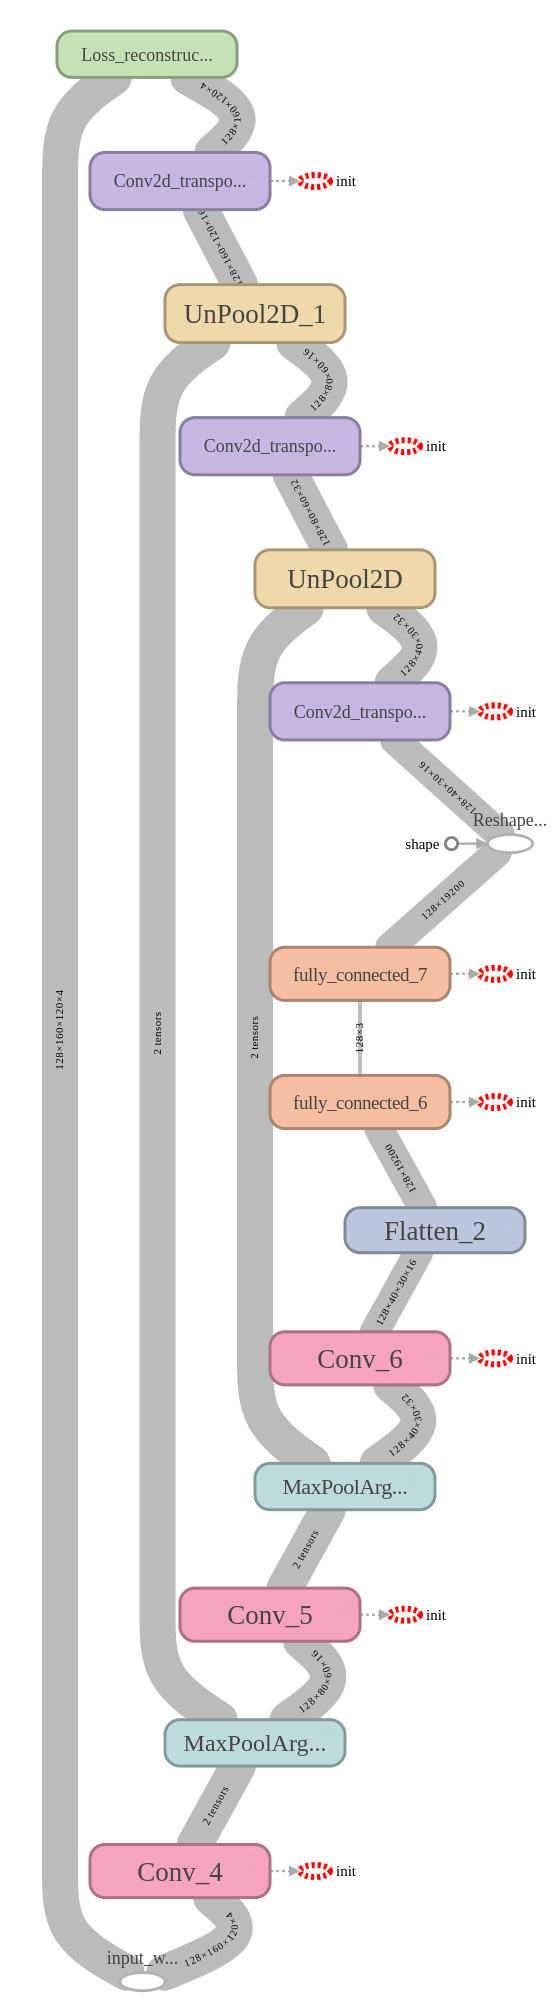
\includegraphics[width=\textwidth,height=\textheight,keepaspectratio]{backbone_2.png}
  \caption{TensorFlow detailed graph representation of a single.}
  \label{fig:tf_graph_2}
\end{figure}

\section{Model pre-training}

Xavier initialization provides good initial parameters to allow robust gradient backpropagation through a deep neural network architecture.
This approach provides alike learning rates for all neurons in the network.
It also decreases the chances of a neuron dying-out during initial training steps.
We can view Xavier initialization as a method, that allows to effectively use a larger number of neurons which is capable of finding a better local minima.

Yet, Xavier initialization does not guarantee, that a good local minima will be found during the training process.
Another robust approach to initialize network weights is reusing the weight of an already trained model.
As, for example, we can initialize model with weights, that has been learned by the same model architecture but on a different dataset \cite{Yosinski2014}.

We have next motivation for model pre-training.
In our early experiments we discovered high instability of the training process.
That is to say, an autoencoder based model learned to produce the same output image regardless of the input.
We assume, that this single output was a solution for minimization of average MSE on the complete training set.

We discovered that this instability can be explained by one of the next 2 factors:
\begin{enumerate}
  \item Extremely high compression rates. Trying to represent 76800 dimensional inputs in a 6- or lower-dimensional space is highly non trivial. Decreasing the compression rate always resulted in a more stable training.
  \item Noisy $L2$ loss. Neighboring pixels of a computer game images often have sharp differences and therefore are less correlated between each other.
  While we are trying to discover spacial structure using pixel-wise means squared error (MSE), such low correlation can be detrimental to the learning process.
  The reason is, that neighboring pixels can look as different from target value as remote pixels of the image.
  Which means that a small errors in the spacial transformations of the data can result in as high error as a large spacial transformations.
  These impedes learning process.
\end{enumerate}
% TODO: insert information about L2 error for neigboring pixels
% Mathieu2015 - MSE issues

From these two issues we can naturally deriver several methods for tackling this problem.
First, we can increase dimensionality of the encoding space, thus decreasing the compression ratio of the data.
Unfortunately, this would negatively effect the goal of this work: extracting low-dimensional interpretable features.
Therefore, we propose to improve the learning process by mitigating the noisy nature of the mean squared error.

We propose a model pre-training procedure that would incentivize learning of spatial information by the feature extractor (encoder).
We suggest, that increasing correlation of the neighboring pixels would result in at least local differentiability of spacial-dependent components of the latent feature space.
This quality should positively impact probability of learning latent representation of, specifically, spacial features by gradient descent.

In particular, we propose using training data to generate inputs for pre-training with higher local correlation between pixels.
We suggest using Gaussian blur as a preprocessing step to produce such data.
Next formula describes the transformation for each pixel of the image:

\begin{equation}
  G(x, y, \sigma) = \frac{1}{2\pi\sigma^2}\exp^{-\frac{x^2+y^2}{2\sigma^2}}
\end{equation}
where $(x, y)$ is relative position of the effected pixel to the source of transformation, $\sigma$ is real-valued parameter of the transformation.

Our pre-training technique is therefore dependent on two parameters: blur $\sigma$ and number of pre-training steps $N$.
We perform pre-training in scheduled way, by decreasing $\sigma$ linearly during the pre-training phase.
This allows smooth adaptation of the model parameters to the actual training data.
Altogether, we summarize our algorithm on listing \ref{alg:pretr}.

% !TEX root = ../thesis.tex

\begin{algorithm}[H]
 \KwData{X  \text{ (Train set)}}
 \KwResult{$\theta \text{ (Learned weights)}$}

 $\textbf{Require: } \sigma\text{: maximum blur distortion value}$

 $\textbf{Require: } N \text{: number of pre-training steps}$

 $\theta \gets \theta_0 \text{ (Xavier Initialization)}$

 \For{i in N}{

  $\sigma_i \gets (1 - \frac{i}{N})*\sigma \text{ (Calculate distortion parameter for current step)}$

  $X_i \gets \text{ Select minibatch examples i.i.d. from $X$}$

  $\hat{X_i} \gets \sigma(X_i, \sigma_i) \text{ (Apply distortion to the minibatch)}$

  $\theta \gets train\_minibatch(\theta, \hat{X_i}) \text{ (Perform a training step using distorted input)}$

 }

 \Return $\theta$

 \caption{Pre-training procedure for spatial-feature extraction}\label{alg:pretr}

\end{algorithm}

% TODO: finish the thought, add some math

\section{Manifold learning}\label{ss:mf}

While Variational Autoencoders and Generative moment matching networks can successfully learn dense data manifold, those models make no assumption about the nature of the manifold space \cite{Li2015, Ren2016, Kingma2013}.
In this section we describe our regularization techniques to incentivize manifold construction in more interpretable form.
For instance, we would like the manifold space to have local resemblance of the Euclidean space.
Also, we prefer to have predictable density of the data in the manifold space.

\subsection{Predictive objective}

With predictive objective we would like to explore the temporal relation of the data.
Training data is represented as one or multiple sequences of images.
Each sequence contains information about some unspecified arbitrary movement of an actor (player) through the environment (game).
This type of data contains at least two structural dependencies: correlation of information within each single image and temporal dependencies between frames.
While structural dependency within a single image is observed by the model at once for each input, temporal relation of the data is not taken into account.
With predictive objective we would like to create additional constrain on the model, that would allow learning of that temporal dependence of the data.

Let's first try to describe minimum necessary number of degrees of freedom.
Let's assume that the environment (a game map, or a building) is fixed, has no moving objects and does not change over time.
In that case we can construct the first person view of player given next inputs:
\begin{enumerate}
  \item $x, y, z$ - axes coordinates of the player within the environment,
  \item $\phi, \theta, \psi$ -  - roll, pitch, yaw angles depending on the orientation of player's view to coordinate axis,
  \item $\alpha$ - angle of players view.
\end{enumerate}

We can safely assume, that angle $\alpha$, as well as other possible output specific parameters, remains constant over the time.
In that case, we have in total 6 variables.
Namely, vectors of actor's view and position.
Lets assemble them into a players parameter vector $p=(x, y, z, \phi, \theta, \psi)$.

Lets make next two assumptions:
\begin{enumerate}
  \item Variables $x, y, z, \phi, \theta, \psi$ are independent from each other in general case.
  \item Function, $p_t=f(t)$, extracting player's positional information over time $t$, is a continuous function.
\end{enumerate}

Let's assume, that encoder part of the network $e(x_t)= \hat{p_t}$, where $x_t$ is an image input at time $t$, successfully reconstructs the trajectory ${x_0, \ldots, x_N}$ on some manifold $M$.
Than we can state, that a local neighborhood of each point on the manifold $\hat{p_t}$ resembles continuous space of vector $p$. That gives us a possibility to apply geometrical operations within a neighborhood.

To add predictive objective we shall rely on the fact, that image at time $t_i$ is statistically dependent on whole sequence of previous images ${t_0, \ldots, t_{i-1}}$.
Given information ${t_0, \ldots, t_{i-1}}$ we can try to predict information about at time $i$.
While in the space of input images this task not trivial, in the space of player parameters $p$ we can simply approximate next position $p_{t+1}$ by current direction.
In other words, we can expect, that next transition of the player during small time period $\epsilon$ would be a lot like previous transition over the same period of time.
If we express it as $p_i = p_{i-1} + \delta_{i-1}$ we can expect that $\delta_i \approx \delta_{i-1}$ for sufficiently small time step. Deriving from that, we can construct next prediction procedure:
\begin{equation}
  \begin{aligned}
    &p_{i+1} = p_i + \delta_i \approx p_i + \delta_{i-1},\\
    &p_i + \delta_{i-1} = p_i + (p_i - p_{i-1}) = 2*p_i - p_{i-1}, \\
    &p_{i+1} \approx 2*p_i - p_{i-1}
  \end{aligned}
\end{equation}

At the same time, for sufficiently small values of $\delta$ we can expect this approximation to hold in the manifold space:
\begin{equation}
  \hat{p}_{i+1} \approx 2*\hat{p}_i - \hat{p}_{i-1}
\end{equation}

This procedure is schematically depicted on figure \ref{fig:m_pred}.

Unfortunately, the discretization of the video stream of the training data does not guarantee sufficiently small transitions between consecutive frames.
This is especially true for changes of the angle of view ($\phi, \theta, \psi$), since they can appear almost instantaneously.

\begin{figure}[h!]
  \centering
    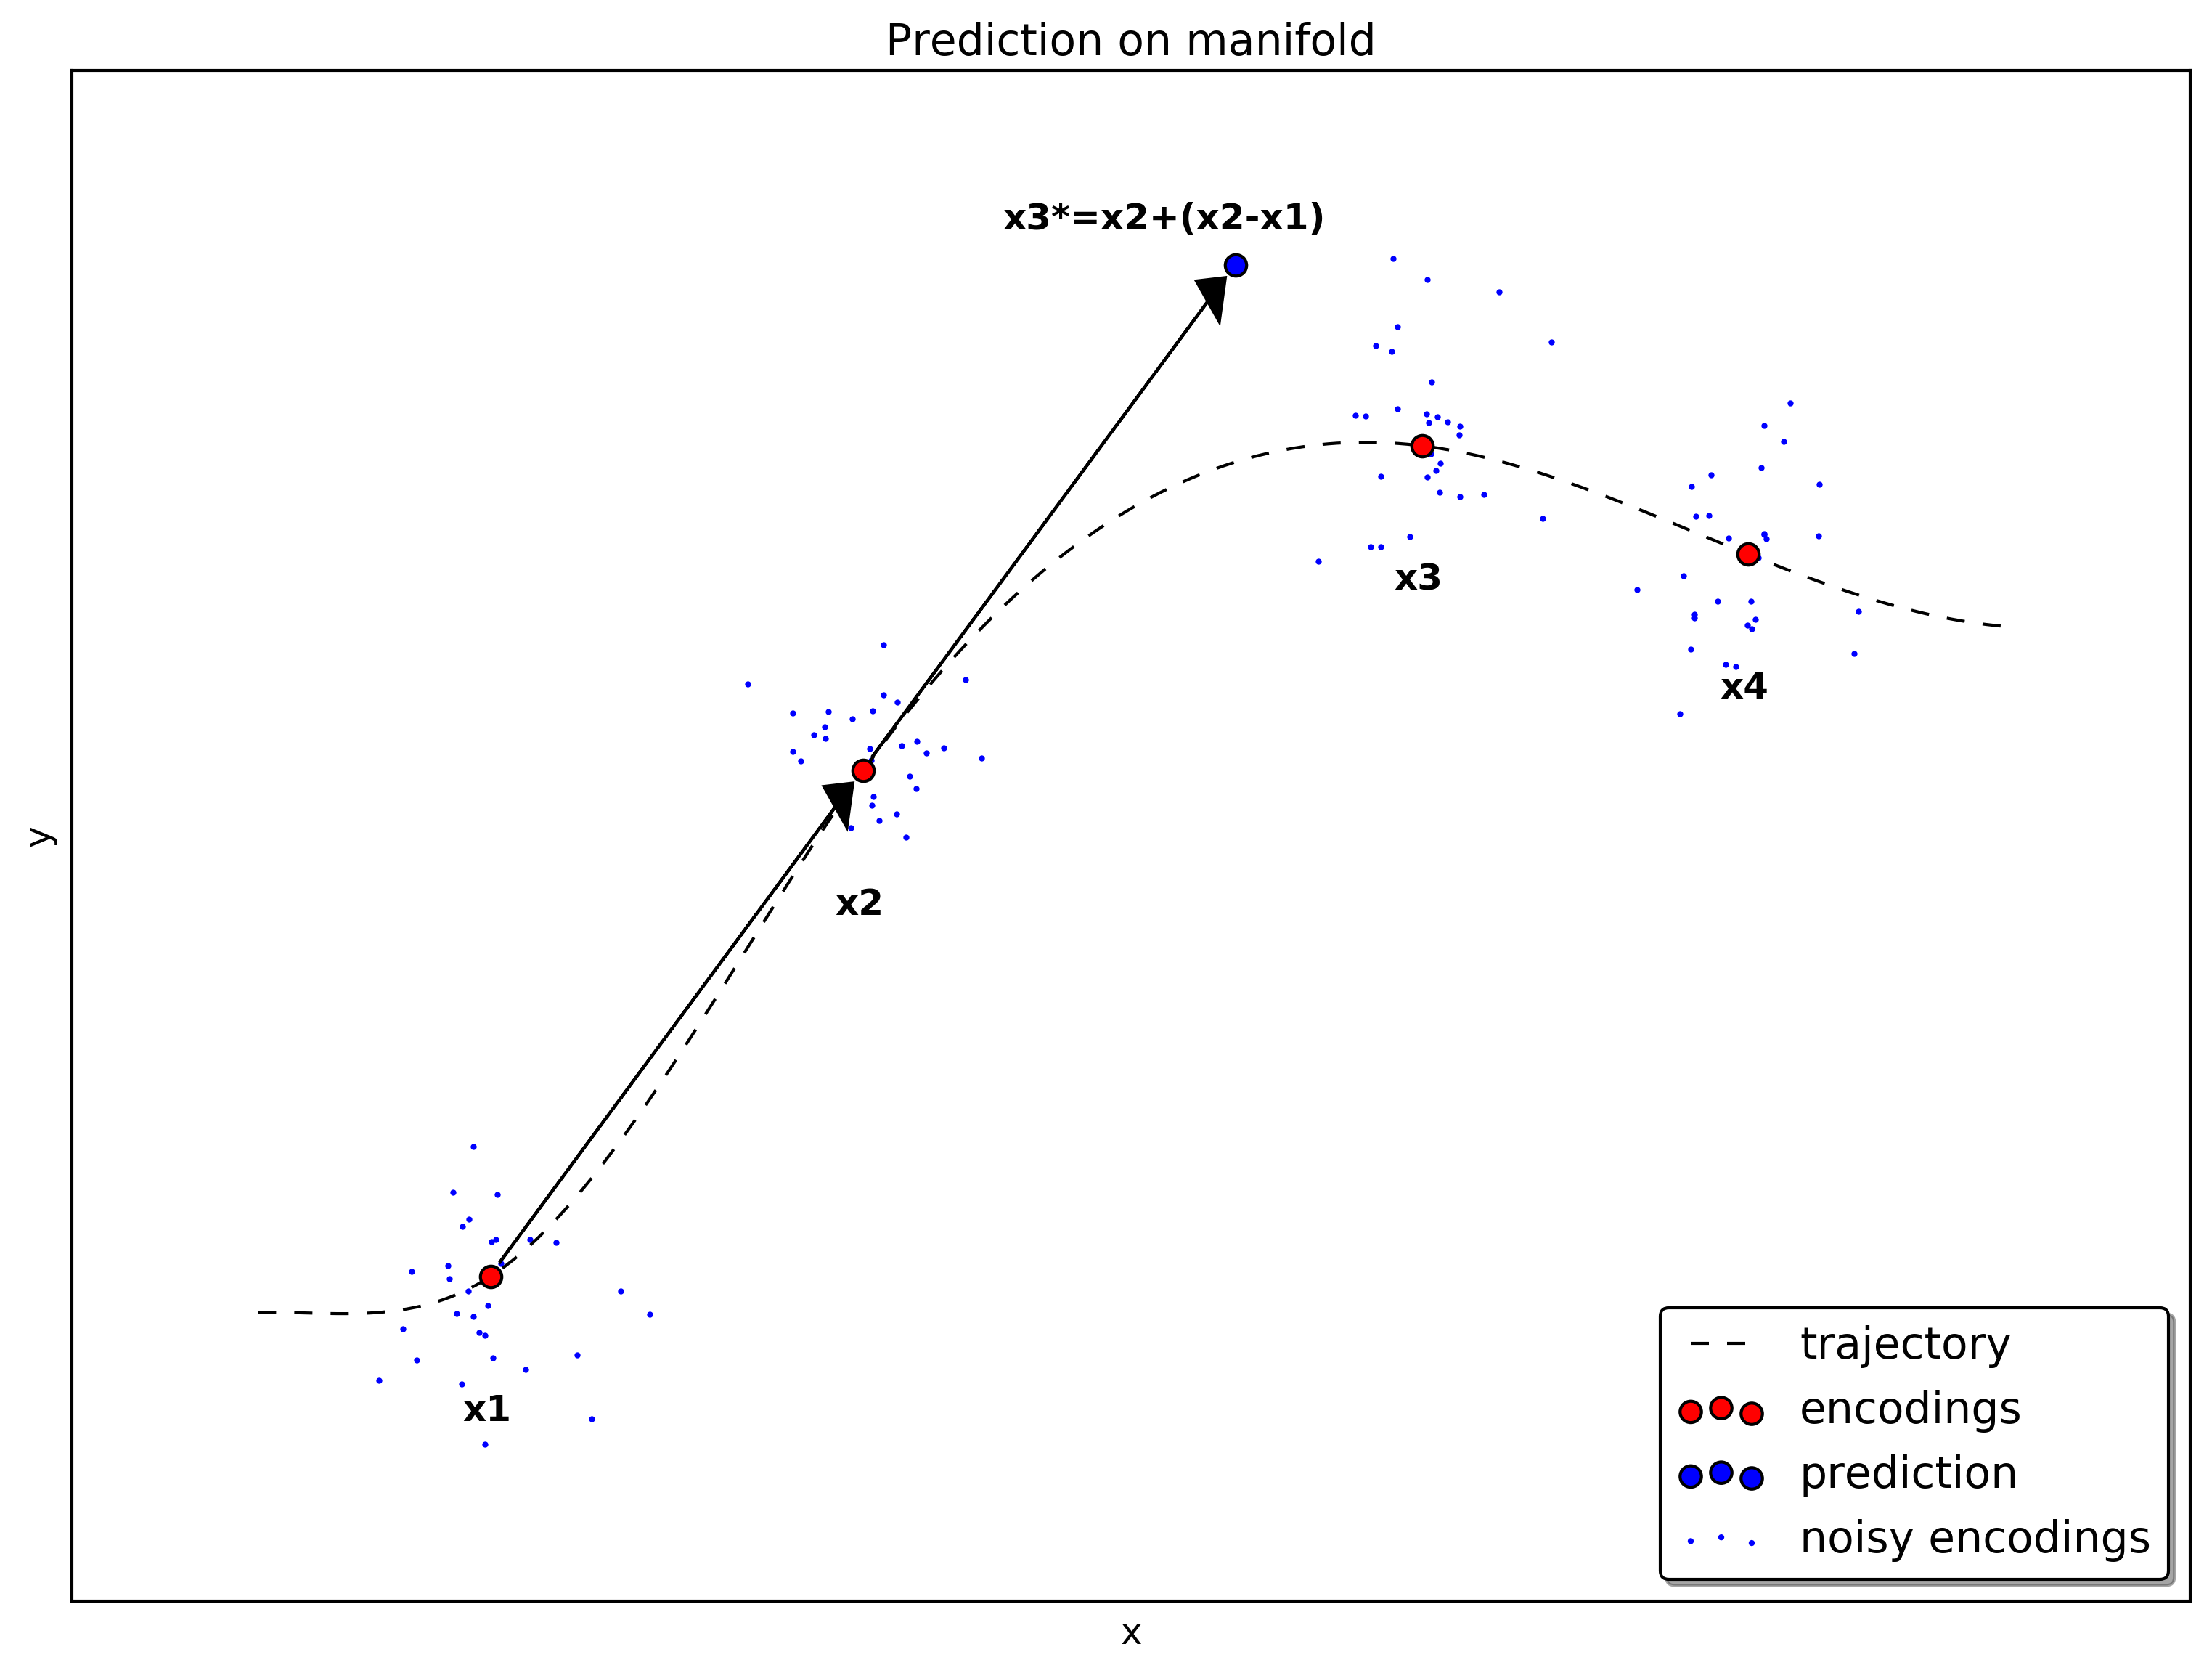
\includegraphics[width=0.85\textwidth,height=0.85\textheight, keepaspectratio]{prediction}
  \caption{Approximating encoding of frame $x_3$ by the encodings of two previous frames $x1, x2$ on the manifold trajectory}.
  \label{fig:m_pred}
\end{figure}

% TODO: add a couple of words about model changes and reconstruction error

\subsection{Denoising regularization}

Early experiments showed largely uneven density of the manifold projection.
In particular cases this led to \textit{lumps} of images concentrated in a small region of the projection space.
Images in the same lump tend to show high similarity between each other.

This behavior can be explained by largely uneven similarity between images across the training set.
For instance, let's says a single step along some trajectory is represented by $N$ discrete time-steps and, therefore, $N$ distinct sequential image inputs.
We can argue, that 2 distinct $N$-sequences from different parts of the trajectory might have highly different variation within the sequence.
As, for example, a single step towards the wall would cause either significant or almost unnoticeable change of the view depending on the distance from the wall.

High contrast of the degree of pair-wise image similarity across the dataset means, that alike errors in determining current position $p_i$ would cause highly uneven reconstruction error $L_{reco}$ depending on position $p_i$.
This, in turn, would lead to smaller gradient values during the learning process.
In the extreme case, gradients produced within regions of high similarity can be comparable or smaller than the noise of gradients of less similar regions.

To resolve this issue we propose using noise injection in the manifold space.
We suggest, that noisy embeddings would allow to enforce a minimum distance between prototypes in the embedding space.
This minimum distance should allow to increase size of the regions around lumps, therefore effectively decreasing density in this regions.
As a result, we expect high density regions to become more robust against gradient noise, produced by different inputs.

% TODO: mathematics here

\subsection{Density regularization}

Despite continuous nature of actors movements, we have access only to discretized data in form of video frames.
This discretization sometimes results in sharp changes in the visual data in subsequent frames, that, in turn, leads to low-density regions in the manifold space.
Within such a region we can not longer argue about local resemblance of the manifold to a Euclidean space, continuous assumption about data at hand does not hold any longer.

Sharp changes in density of the manifold make it harder to argue about interpretability and quality of the learned concepts. Furthermore, our experiments has shown, that manifolds with large number of low density regions tend to create larger number of self intersections, further complicating the interpretation of the learned features.

We, therefore propose a low-density regularization to account for regions with sharp changes.
We suggest using an additional error term during the training phase to penalize large distances between consecutive frames, therefore dragging them closer together.
Such regularization would compete with the reconstruction objective of the autoencoder network.
But our main interest is interpretable feature extraction, not archiving perfect reconstruction of the images.

Therefore, we calculate euclidean distance between pair of subsequent images:
\begin{equation*}
d(x_t, x_{t+1}) = \Big(\sum^i { (x_{t,i}-x_{t+1, i})^2}\Big)^{\frac{1}{2}}
\end{equation*}
And penalize distances exceeding certain constant value $d_{max}$:

\begin{equation*}
  L_{dens} = \gamma*\max(0, d(x_t, x_{t+1})-d_{max})
\end{equation*}
where $\gamma$ is a constant parameter defining contribution of the density regularization in total loss.


Figure \ref{fig:model} summarizes our modification to the autoencoder architecture on a single schema.

% !TEX root = ../thesis.tex

\begin{figure}

\centering
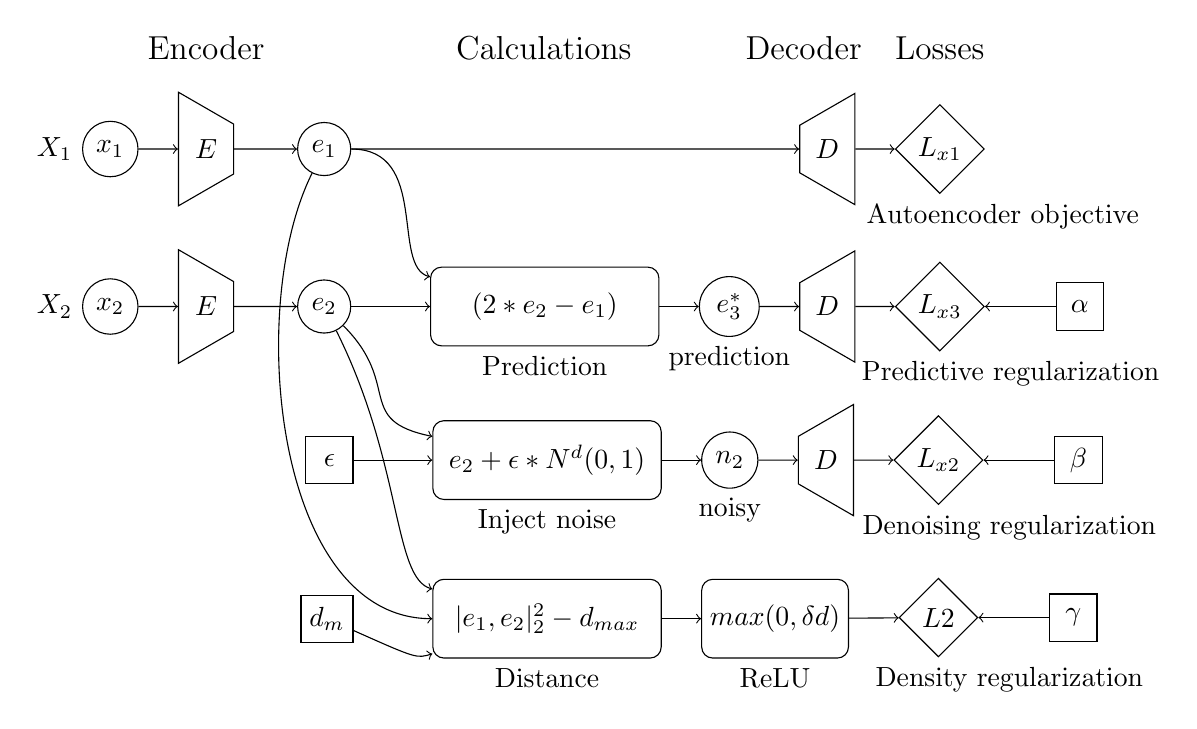
\begin{tikzpicture}
%   [align=center,node distance=2cm]
  [
    every label/.style={align=center},
  	lbl/.style={draw, circle, minimum width=0mm, minimum height=0mm, inner sep=0pt},
    vlbl/.style={draw, circle, minimum width=0mm, minimum height=0mm, inner sep=0pt},
    state/.style={draw, circle, minimum width=6mm, minimum height=6mm, inner sep=3pt},
    param/.style={draw, rectangle, minimum width=6mm, minimum height=6mm, inner sep=3pt},
    func/.style={draw, rectangle, minimum width=2.9cm, minimum height=1cm, inner sep=3pt, rounded corners},
    relu/.style={draw, rectangle, minimum width=1cm, minimum height=1cm, inner sep=3pt, rounded corners},
    enc/.style={draw, trapezium, shape border rotate=-180, minimum width=0.7cm, minimum height=0.7cm, inner sep=2pt},
    dec/.style={draw, trapezium, shape border rotate=90,  minimum width=0.7cm, minimum height=0.7cm, inner sep=2pt},
    loss/.style={draw, diamond, minimum width=1cm, minimum height=1cm, inner sep=2pt},
    node distance=20mm,
    classical/.style={dashed,->,shorten >=4pt,shorten <=4pt,>=stealth},
    % Define arrow style
    pil/.style={
           ->,
           thick,
           shorten <=2pt,
           shorten >=2pt,}
%     dotted/.style={dotted,-,shorten >=4pt,shorten <=4pt,>=stealth}
  ]
%   \node (x) [state, label=left:$X_1$] {$x_1$};
  \node (x1) [state, label=left:$X_1$] {$x_1$};
  \node (x2) [state, below of=x1,label=left:$X_2$] {$x_2$};
  \node (enc1) [enc, right=.5cm of x1] {$E$};
  \node (enc2) [enc, right=.5cm of x2] {$E$};
  \node (e1) [state, right of=enc1,shift={(-0.5,0)}] {$e_1$};
  \node (e2) [state, right of=enc2,shift={(-0.5,0)}] {$e_2$};

%   prediction
  \node (pred) [func, right=1.0cm of e2,label=below:Prediction] {$(2*e_2-e_1)$};
  \node (e3) [state, right=.5cm of pred,label=below:prediction] {$e_3^*$};

%   noise
  \node (noise) [func, below right=1.2cm and 1.13cm of e2, label=below:Inject noise] {$e_2 + \epsilon*N^d(0, 1)$};
  \node (n2) [state, right=.5cm of noise,label=below:noisy] {$n_2$};
  \node (eps) [param, left=1.cm of noise] {$\epsilon$};

%   distance
  \node (dist) [func, below=1cm of noise,label=below:Distance] { $\text{  }|e_1, e_2|_2^2-d_{max}\text{  }$ };
%   \node (d) [state, right=.5cm of dist,label=below:distance] {$\delta d$};
  \node (rel) [relu, right=0.5cm of dist,label=below:ReLU] {$max(0,\delta d )$};
  \node (dmin) [param, left=1.cm of dist] {$d_{m}$};

%   decoding
  \node (decp) [dec, right=.5cm of e3] {$D$};
  \node (dec2) [dec, above of=decp] {$D$};
  \node (decn) [dec, right=.5cm of n2] {$D$};

  \node(l2)[loss, right=.5cm of dec2, label={[xshift=0.8cm]below:{Autoencoder objective}}]{$L_{x1}$};
  \node(lp)[loss, right=.5cm of decp, label={[xshift=0.9cm]below:{Predictive regularization}}]{$L_{x3}$};
  \node(ln)[loss, right=.5cm of decn, label={[xshift=0.9cm]below:{Denoising regularization}}]{$L_{x2}$};
  \node(ld)[loss, below of=ln, label={[xshift=0.9cm]below:{Density regularization}}]{$L2$};


%   \node (le3) [state, right of=lp] {$x_3$};
%   \node (le2_1) [state, right of=l2] {$x_2$};
%   \node (le2_2) [state, right of=ln] {$x_2$};

  \node (a) [param, right=.9cm of lp] {$\alpha$};
  \node (b) [param, right=.9cm of ln] {$\beta$};
  \node (g) [param, right=.9cm of ld] {$\gamma$};

%   labels
  \node (lbl2) [lbl, above of=enc1, yshift=-1cm, label=above:\large{Encoder}]{};
%   \node (lbl3) [lbl, left of=lbl2,label=above:\large{Inputs}]{};
  \node (lbl5) [lbl, above of=l2, yshift=-1cm, label=above:\large{Losses}]{};
  \node (lbl4) [lbl, above of=dec2, yshift=-1cm, xshift=-0.3cm, label=above:\large{Decoder}]{};
  \node (lblx) [lbl, left of=lbl4]{};
  \node (lbl1) [lbl,left of=lblx, xshift=0.7cm,label=above:\large{Calculations}]{};
%   \node (lbl6) [lbl, right of=lbl5, label=above:\large{Parameters}]{};

%   \node (vlbl_p) [vlbl, right of=a, label={[xshift=.5cm]left:\rotatebox{-90}{\large{Predictive}}}]{};
%   \node (vlbl_ae) [vlbl, above of=vlbl_p, label={[xshift=-.5cm]left:\rotatebox{-90}{\large{Autoencoder}}}]{};
%   \node (vlbl_n) [vlbl, below of=vlbl_p,label={[xshift=-0.5cm, align=center]left:{\rotatebox{-90}{\large{Denoising}}}}]{};
%   \node (vlbl_d) [vlbl, below of=vlbl_n, label={[xshift=.5cm]left:\rotatebox{-90}{\large{Density}}}]{};


%   arrows
%   \draw[->] (description) .. controls ([xshift=-4cm] description) and ([xshift=4cm] text) .. (text);
  \draw[->] (e2) .. controls ([xshift=1cm, yshift=-2cm] e2) and ([xshift=-.5cm] dist.north west) .. (dist);
  \draw[->] (e2) .. controls ([xshift=1cm, yshift=-1cm] e2) and ([xshift=-1cm] noise.north west) .. (noise);

  \draw[->] (e1) .. controls ([xshift=1cm] e1.east) and ([xshift=-.5cm] pred.north west) .. (pred);
  \draw[->] (e1) .. controls ([xshift=-1cm, yshift=-2cm] e1) and ([xshift=-2.0cm] dist.west) .. (dist);


  \draw[->] (x2) -- (enc2);
  \draw[->] (enc2) -- (e2);
  \draw[->] (e2) -- (pred);
  \draw[->] (pred) -- (e3);
  \draw[->] (e3) -- (decp);
  \draw[->] (decp) -- (lp);
%   \draw[->] (le3) -- (lp);
	\draw[->] (a) -- (lp);

  \draw[->] (x1) -- (enc1);
  \draw[->] (enc1) -- (e1);
  \draw[->] (e1) -- (dec2);
  \draw[->] (dec2) -- (l2);
%   \draw[->] (le2_1) -- (l2);
	\draw[->] (b) -- (ln);

%   \draw[->] (dist) -- (d);
%   \draw[->] (d) -- (rel);
  \draw[->] (dist) -- (rel);
  \draw[->] (rel) -- (ld);

  \draw[->] (noise) -- (n2);
  \draw[->] (n2) -- (decn);
  \draw[->] (decn) -- (ln);
%   \draw[->] (le2_2) -- (ln);
  \draw[->] (g) -- (ld);

  \draw[->] (eps) -- (noise);
  \draw[->] (dmin) .. controls ([xshift=-.2cm] dist.south west) .. (dist);



%   	\draw [color=gray,thick](-1.5,-1) rectangle (15.5,1.5);
% 	\node at (-0.5,1) [above=5mm, right=0mm] {\textsc{first-order noise shaper}};
% 	\draw [color=gray,thick](-0.5,-9) rectangle (12.5,-5);
% 	\node at (-0.5,-9) [below=5mm, right=0mm] {\textsc{second-order noise shaper}};

%   \coordinate (aux) at (x1.south) -- (x1.south|-x2.north);
%   \draw[dashed]([xshift=-1cm]x1.north west|-aux) -- ([xshift=1cm]x2.north east|-aux);


%   \draw (0,-1) -- (4,-1);
\end{tikzpicture}
\caption{Spacial feature extractor with regularization terms.}
\label{fig:model}
\end{figure}


% !TEX root = ./thesis.tex

\chapter{Evaluation}
\label{ch:eval}

Finding a definite good evaluation method for unsupervised models is a long-standing and inherent problem \cite{Li2015}. In this section we describe our evaluation techniques along with data collection process. We introduce two task-independent metrics to evaluate the qualities of the extracted manifold. Further we discuss possible applications of the model to real-world data.


\section{Evaluation data}
\subsection{Data collection}

Access to large amount of training data is crucial for applying deep learning models.
Successes of deep learning on image recognition and segmentation tasks can be attributed to existence of large research datasets as ILSVRC and Places365 \cite{ILSVRC15, Zhou2016} containing millions of labeled images.
Machine translation, NLP tasks \cite{Karpathy2014, Kim2014} often rely on low-dimensional word embedding models.
Such models, as for example as word2vec or Glove \cite{Mikolov2013, pennington2014glove}, are trained on terabytes of textual data.
Deep reinforcement models might use existing gaming engines to generate required training data "on the go".
As, for example Google DeepMind team uses Atari 2D games to generate data for Q-learning \cite{Mnih2013}.

For the purpose of this research we collect visual data using the ViZDoom AI research platform \cite{Kempka2016}.
ViZDoom is a Doom-based platform for reinforcement learning.
It provides access to raw visual data from the Doom gaming engine.
Doom is a first-person shooter (FPS) computer game utilizing 3D graphics.
In context of our research the ViZDoom platform allows automatic visual data generation and collection.
Example of the output image is shown on figure \ref{fig:doom}.

We created multiple \texttt{Doom II} maps specifically for our task using the Slade \cite{Slade3} software.
Created maps provide high diversity of textures for better discrimination between images, captured from different positions on the map.
Other reason for diverse structures on the map is to explicitly brake symmetry of the map.
Symmetric maps look alike from different player positions which leads to entangled manifolds in feature space.
Such position tend to be encoded with the same values of sparse features.
This represents a difficulty for evaluation and comparison of quality of sparse features.

We record multiple movement trajectories on each map.
More specifically, we record 10000-300000 consecutive images of unstructured movement of the player on the map for training purposes.
In addition to that, we record movement along well defined structured trajectories as a "circle" or an "eight" for model evaluation and comparison of quality of extracted features.


\begin{figure}
\centering
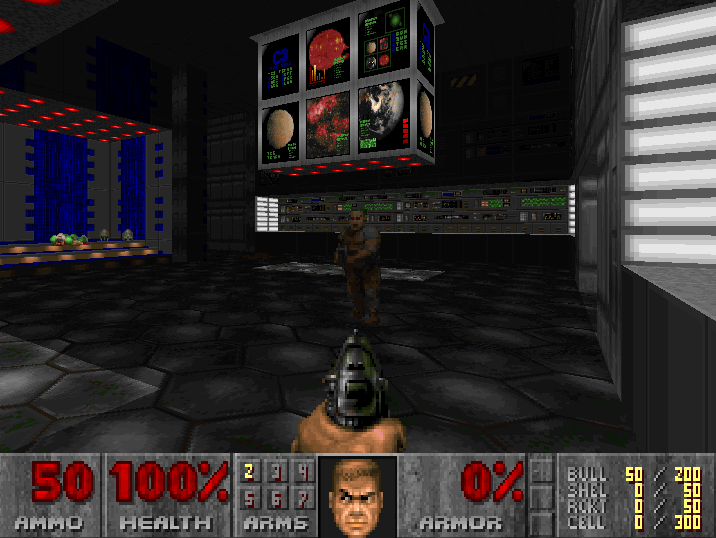
\includegraphics[width=.80\textwidth]{doom.png} %{CS0031}
\caption{Example of \texttt{Doom II} image collected with ViZDoom \cite{Kempka2016}.}
\label{fig:doom}
\end{figure}

\subsection{Dataset description}

We collect multiple sets of visual data with varying complexity of players movement.
We can specify next 3 classes of trajectories used either for training or evaluation:
\begin{itemize}
  \item Continuous closed trajectory without intersection. A circular movement is one example of such trajectory.
  \item Continuous closed trajectory with intersection. An \text{eight} is an example of such trajectory.
  \item Continuous random movement across the environment (map).
\end{itemize}

Furthermore, we introduce multiple complexity levels of movement across trajectories by reducing degrees of freedom of such movements:
\begin{itemize}
  \item Most restricted. Only movement along a single axis at a time is possible. This category includes movements across rectangular trajectories while maintaining fixed direction of the view or changing the direction of the view while standing still. This category provides includes trajectories of the lowest complexity.
  \item Less restricted. Multiple degrees of freedom at a time allowed. For example, movement along multiple axis facing one direction or forward movement while changing the direction of the view.
  \item Free movement across the map with no restrictions.
\end{itemize}


\subsection{Data format}

We collect RGBD images from the 3D engine. Each image has resolution of 160 by 120 pixels. Each pixel is describe by 3 color channels and a single distance channel. Each channel can take a discrete value between 0 and 255 including. This format results in 76800 dimensional inputs.


\section{Predictive evaluation} \label{ss:score}

Evaluation of the performance of unsupervised models is inherently difficult.
Discriminative models typically use well-defined metrics with clear quantifiable outputs, as classification accuracy, F-measure etc. Unsupervised models generally have no access to such metrics.
Solutions for some under-defined objectives, as finding image super-resolution or generating new data samples, can be evaluated by involving manual human grading, which is costly and time-consuming \cite{Dahl2017, Goodfellow2014}.
Other models rely on the primary learning objective, which is not necessarily representative of the actual model performance. As, for example, minimizing MSE for image comparison can result in low-quality blurry results, or matching certain characteristics of natural probability distribution in a generative process does not guarantee realistically looking generated data \cite{Li2015, Mathieu2015}. At last, some unsupervised learning techniques can be evaluated through performance on real world tasks by showing, that results of unsupervised learning can improve performance of discriminative models. For example, reusing network weights of denoising and contractive autoencoders led to improved classification results \cite{Rifai2011, Vincent2010}, as well reusing weights of word embeddings \cite{NIPS2013_5021} led to increased performance on a number of natural language processing tasks.

In context of this work we would like to have access to a concise measure for comparison of model designs.
Primary objective of an autoencoder -- good reconstruction of the input image -- is not very descriptive, since it makes no assumption about the spatial characteristics of the extracted features. Nevertheless, we provide our reconstruction loss values with the experiments.

We are going to use \textit{predictive score} as a main mean of model comparison from perspective of spatial feature extraction. With the predictive objective we would like to evaluate the quality of extracted spatial features. We do that by considering local resemblance of the manifold to an euclidean space. But, since we are working with unlabeled data another assumption is required. Namely, for any trajectory of actors movement we expect, that the best approximation of the transition between current and next step to be equivalent to the transition between previous and current step (when only last two frames are available for performing the prediction). We, therefore try to predict spatial position of the player on the next step on the manifold calculating it as $\hat{x}_{t+1} = x_t + (x_t- x_{t-1})$. Figure \ref{fig:m_pred} illustrates the process.
Since different models have different deformations of manifold space and, therefore, might differ in terms of absolute values of the $L_2$ loss between predicted and actual location $L_2(\hat{x}_{t+1}, x_{t+1})$, we use relative improvement as a reference. We compare the improvement of prediction over a naive prediction $\tilde{x}_{t+1} = x_t$. We therefore define predictive metric as follows:
\begin{equation}
  \begin{aligned}
  &P_{L2}(X) = \frac{1}{N-2}\sum^{N-1}_{i=2}{f(L_2(\hat{x}_{i+1}, x_{i+1})}, {L_2(x_i, x_{i+1}))}\\
  &f(x, y) = max(0, \frac{y-x}{y}) \text{ note: } f(x, y) \in [0, 1]
  \end{aligned}
\end{equation}
where $N$ is a number of inputs in the validation set. Note, that $P_{L2}(X) \in [0, 1]$ and 1.0 indicates perfect prediction of the next frame at each moment in time; 0.0 average prediction to be worse than naive prediction. Prediction is possible only for elements starting from the 3rd, therefore first two images do not contribute to the score.

Note, that similar technique is used as a model regularization. Yet, predictive regularization is applied as a reconstruction error and does not have direct effect on the predictive score. For example, an decoder of large enough capacity can have very low reconstruction error of both actual encoding $x_{t+1}$ and predictive encoding $\hat{x}_{t+1}$, but low score of predictive evaluation. This can happen when two prototypes in the embedding space $x_{t+1}$ and $\hat{x}_{t+1}$ have distinct difference, but are still reconstructed as alike images. This case can be explained by overfitting in the decoder network.

To counter high sensitivity of the $L_2$ error function to outliers we also calculate another flavor of the described evaluation: \textit{binary predictive score}. The total $L_2$ loss value on the complete validation set can increase sharply with presence of outliers. In this case, while overall quality of the manifold might have desired properties for majority of the inputs, it can still produce high validation error. This can happen since $L_2$ error does not take into account varying density of the manifold. To counter that, we introduce a similar simplified version of predictive score, namely producing its binary form. Binary predictive score simply compares the distance between \textit{naive prediction} naive and estimate of the future frame and the prediction calculated by the previous 2 frames.

\begin{equation}
  \begin{aligned}
  & P_{NN}(X) = \frac{1}{N-2}\sum^{N-1}_{i=2}{g  \big( L_2(\hat{x}_{i+1}, x_{i+1})} - {L_2(x_i, x_{i+1}) \big) },\\
  & g(x) = \begin{cases} 1, & \mbox{if } x > 0 \\ 0, & \mbox{if } x \leq 0 \end{cases}
\end{aligned}
\end{equation}
 Value of $P_{L2}(X)$ belongs to interval $[0, 1]$ and 1.0 indicates that calculated prediction for each point was better than naive prediction; 0.0 indicates that no predicted value was better than naive prediction. Perfect score might not be achievable even for some trajectories.

\subsection{Preserving nearest neighbor relation}

Another key characteristic of the desired encoding function is high interpretability of the feature manifold.
Interpretability itself is a loosely defined characteristic. Yet, we propose an evaluation score, that should asses some features of an interpretable spatial manifold. Namely, we argue, that less entangled manifold provide grater interpretability and are more visually appealing. As a proxy measure of such quality we propose exploring nearest-neighbor relation in the input data. We expect, that on a smooth and dense manifold subsequent video frames will be closer to each other than to more remote frames. We therefore can measure, how many subsequent frames remain nearest neighbor in the manifold space. We expect such a characteristic degrade with more entangled and less smooth manifolds.



\begin{equation}
  \begin{aligned}
  & P_{\tau}(X) = \frac{1}{N-2}\sum^{N-1}_{i=2}{\tau  \big(i, m_i, n_i) },\\
  & \tau(i, m, n) =
\begin{cases}
  1, & \mbox{if } (i-1) \in \{m, n\}  \mbox{ and }  (i+1) \in \{m, n\}  \\
  0, & \mbox{if } (i-1) \notin \{m, n\}  \mbox{ and }  (i+1) \notin \{m, n\} \\
  0.5, & \mbox{otherwise }
\end{cases}
\end{aligned}
\end{equation}
where $m_i, n_i$ are indexes of top-2 nearest neighbors of element $i$.  $P_{\tau}(X)$ can take values in interval $[0, 1]$ and 1.0 means that every nearest frame at every time stamp $i$ is the nearest neighbor of the current frame in the embedding space. Value 1.0 might not be achievable, depending on the trajectory.


\section{Model comparison}

In this section we evaluate proposed models. We analyze qualities of the different models in terms of our evaluation scores. We compare performance on datasets of various complexities and analyze sensitivity to different kinds of regularizations.

\subsection{Backbone model comparison}

As a first experiment we would like to asses model behavior on a simple concept, that can be easily understood visually. For that purpose we stick low dimensional encoding in percept able 3D space. This limitation leaves us in the domain of low-complexity trajectories, that depend only on few components. Since one degree of freedom - vertical movement of players view during horizontal motion - is taken, we choose a dataset that explores only 2 degrees of freedom. We also choose a simplest type of trajectory to observe behavior on a trivial task.

First experiment is performed on a closed trajectory with intersections 'eight' that allows only movements along the axis. Player always faces the same direction, therefore we can expect components, describing direction of the view to remain fixed. Following the trajectory player makes several steps along the already visited path (see figure \ref{fig:model_reco}$(a)$). In total, dataset contain 13680 sequential images that corresponds to 3 passes along the trajectory. With this trajectory would like to asses next qualities of the embedding space:
\begin{enumerate}
  \item tractable continuous changes in the embedding over time;
  \item presence or absence of key elements of the trajectory: direction changes;
  \item existence of intersections and coherence of the intersections to the actual trajectory;
  \item visual recognizability of the trajectory in the embedding.
\end{enumerate}

Results of the experiments for 3 backbone models are shown on figure \ref{fig:model_reco}. Metrics of section \label{fig:model_reco} are calculated and mentioned in table \ref{tab:3demb}.


\begin{table}
\begin{center}
    \begin{tabular}{| l | l | l | l | l |}
    \hline
    Model  &  $P_{L2}$    &  $P_{\beta}$     &  $P_{\tau}$ &  $L_{reco}$ \\ \hline
    Fully Connected	 AE  & 0.498 & 0.728 & 0.750 & 54.40        \\
    CNN AE 	 & 0.374 & 0.632 & 0.780 & 49.60        \\
    What-Where AE 	   & 0.000 & 0.403 & 0.623 & 1.50         \\ \hline
    \end{tabular}
\end{center}
  \caption{Comparison of 3 backbone architecture performance on an artificial low-complexity trajectory. Scores   $P_{L2}$, $P_{\beta}$, $P_{\tau}$ are described in section \ref{ss:score} (higher is better). Reconstruction error $L_{reco}$ indicates quality of the image produced by the autoencoder (lower is better).}
  \label{tab:3demb}
\end{table}

\begin{figure}[t!]
	\centering
	\subfigure[Reference \textit{trivial} trajectory]{
  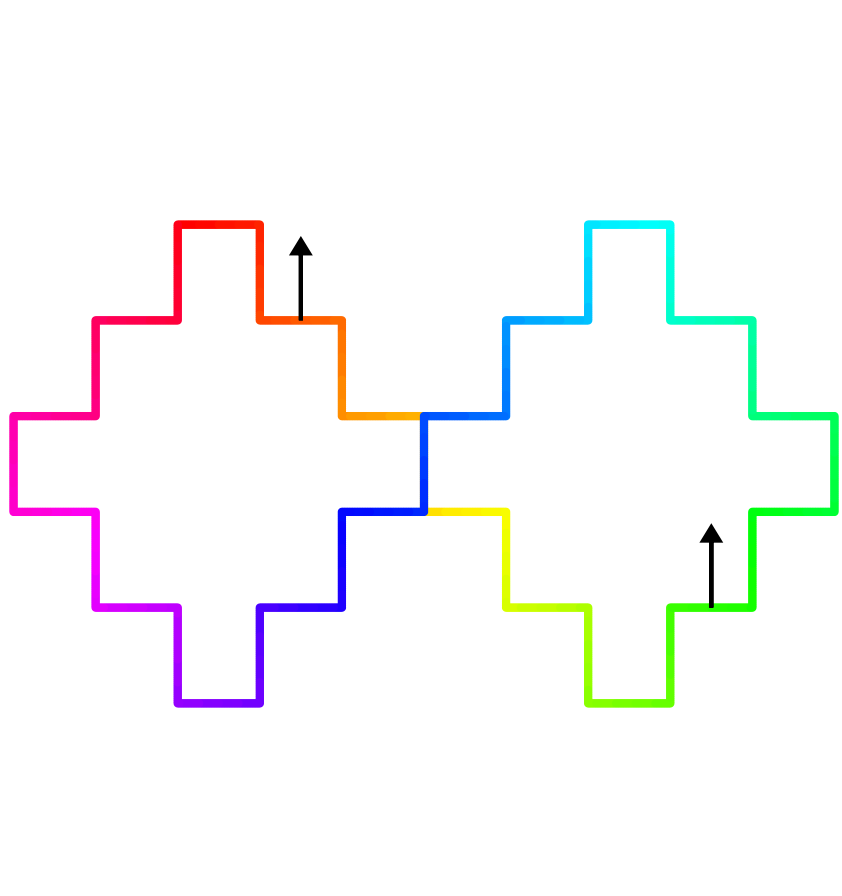
\includegraphics[width=.45\textwidth]{cmp2/tr1.png}
	}
	\subfigure[Embedding with a Fully connected AE.]{
		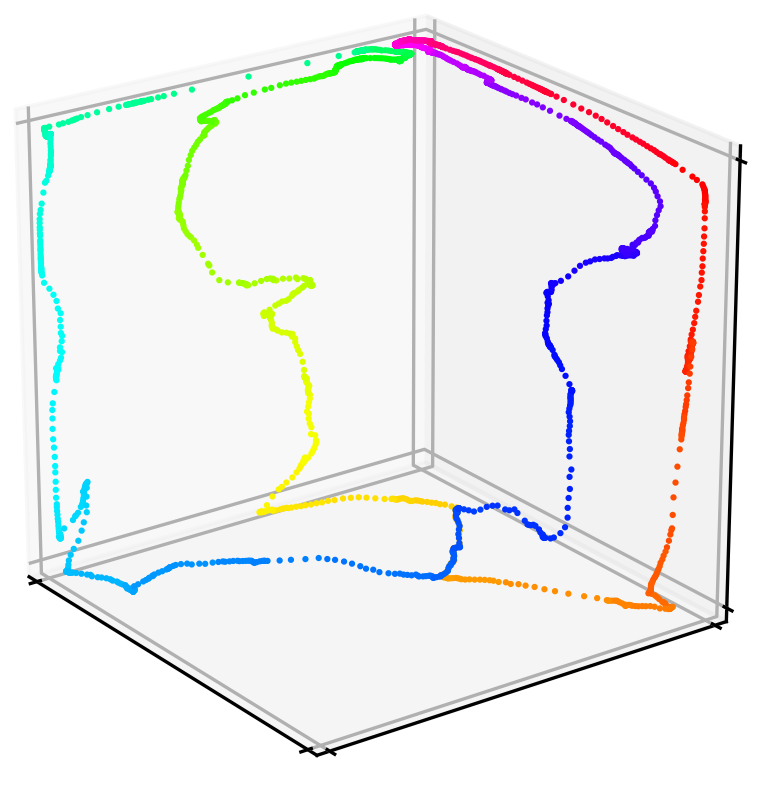
\includegraphics[width=.45\textwidth]{cmp2/fc_3.png}
	}\\
	\subfigure[Embedding with a Convolutions AE.]{
    	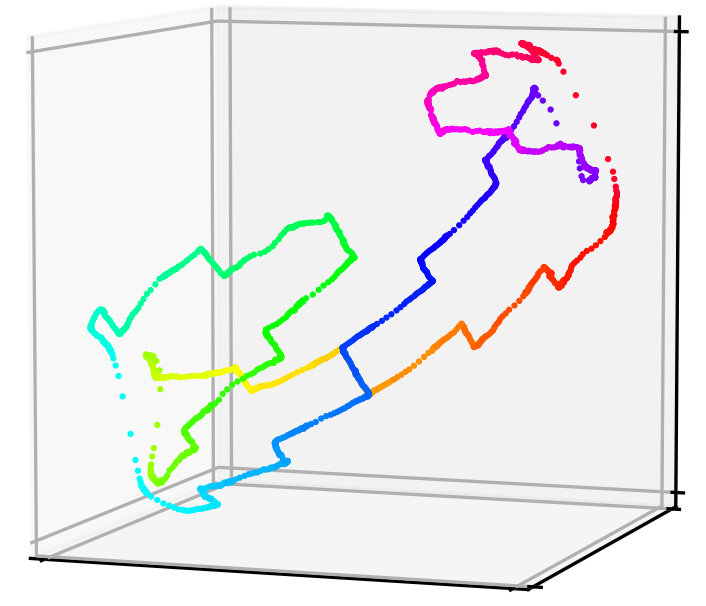
\includegraphics[width=.45\textwidth]{cmp2/cnn_3.png}
	}
	\subfigure[Embedding with the What-Where AE.]{
    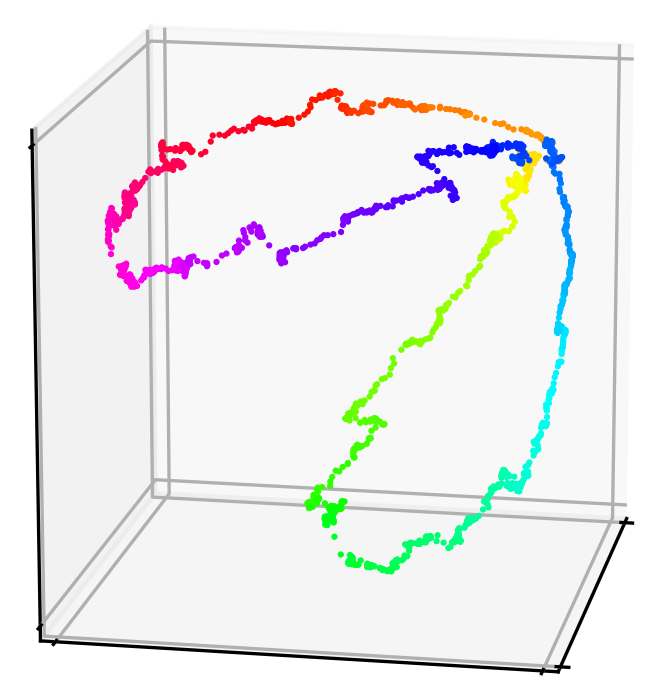
\includegraphics[width=.45\textwidth]{cmp2/ww_3.png}
	}
    	\caption{Embedding a trivial closed self-intersecting trajectory $(a)$ with 2 degrees of freedom using reference models $(b, c, d)$ in a 3-dimensional space. Subsequent frames of the input image sequence are encoded in similar colors to indicate temporal relation between visually disconnected discrete inputs in the embedding space. Color is consistent among the models and corresponds to same points of the trajectory.}
    	\label{fig:model_reco}
\end{figure}

From perspective of the metrics described in section \ref{ss:score} models distinguish sharply. What-Where AE model, while yielding best reconstructions, produced lowest quality embedding space. Average prediction were of a worth quality than using current position as an estimator and only 40\% of the predictions were closer to the actual position of the next frame than current frame. All models were able to maintain more than 63\% of nearest neighbor relations between frames with Convolutional model showing slightly better results than others. Fully connected model produced embedding of the highest predictive power, showing best predictive scores $P_{L2}, P_{\beta}$.

Visual harassment of the embedded trajectories \label{fig:model_reco} shows, that all models were able to preserve somewhat continuous form of the trajectory. All models were able to maintain model elements as intersection and direction changes in some form. Comparing embedding spaces we can see, that embedding produces by What-Where AE falls behind the other models. This observation is coherent with numerical scores calculated above. What-Where AE were able to produce the least complex manifold structure among 3 models. Yet, we are going to ignore this model in future experiments, since with higher dimensional and more complex concepts performance drops sharply and visual assessment is not longer possible without using specialized visualization techniques.

Convolutional model produced the most visually pleasing results. It falls behind the fully-connected model in terms of the synthetic scores, but saw steady improvement with the increase of network capacity (namely, increased size of the feature maps in the layers) and were only limited by our computational resources. Convolutional model was able maintain visually parallel lines of the input trajectory and maintain larger distance between parts of the trajectory. Fully convolutional model appears to spread the trajectory embedding along the surface of the embedding space.

\subsection{Effects of regularization}

In this subsection we try to analyze effects of the regularization on the qualities of the extracted manifold. This time we use a more complex trajectory. Since visual assessment is not a goal of this experiment, we can safely use higher dimensional embedding space. For this experiment we use a natural closed trajectory with single intersection "eight" where player always faces the direction of the movement. This trajectory corresponds to a more natural type of players movement and involves more complex between-frame transformations caused by changing the direction of the view. Sample of the trajectory and regularization are shown on figure \ref{fig:model_param}.

\begin{table}
\begin{center}
    \begin{tabular}{| l | l | l | l | l | l | l | l |}
    \hline
    \multirow{2}{*}{Regularization}      &\multicolumn{3}{|c|}{Parameters} & \multicolumn{4}{|c|}{Scores}  \\   \cline{2-8}

     & $\alpha$ & $\beta$ & $\gamma$    &  $P_{L2}$ & $P_{\beta}$ & $P_{\tau}$ & $L_{reco}$ \\ \hline

		No regularization 	& 0    & 0 & 0 & 0.000 & 0.418 & 0.617 & 60.64 \\ \hline
		Predictive          & 100  & 0 & 0 & 0.052 & 0.614 & 0.738 &  \textbf{57.46} \\
		Denoising           & 0    & 0.0005 & 0 & 0.078 & 0.648 & 0.750 & 61.84 \\
		Distance            & 0    & 0 & 50 & 0.063 & 0.623 & 0.739 & 59.62 \\ \hline
    Predictive and denoising 	& 100    & 0.0005 & 0 & 0.069 & 0.653 & 0.751 & 61.57 \\
    Predictive and distance  & 100    & 0 & 50 & \textbf{0.591} & \textbf{0.909} & \textbf{0.912} & 61.19 \\
    Denoising and distance  & 0    & 0.0005 & 50 & 0.081 & 0.649 & 0.758 & 60.16 \\ \hline
    All 3 & 100    & 0.0005 & 50 & \textbf{0.591} & 0.905 & 0.911 & 62.04 \\ \hline
    \end{tabular}
\end{center}
  \caption{Regularization effects.}
  \label{tab:8emb}
\end{table}

\begin{figure}[t!]
	\centering

	\subfigure[Reference \textit{eight} trajectory]{
  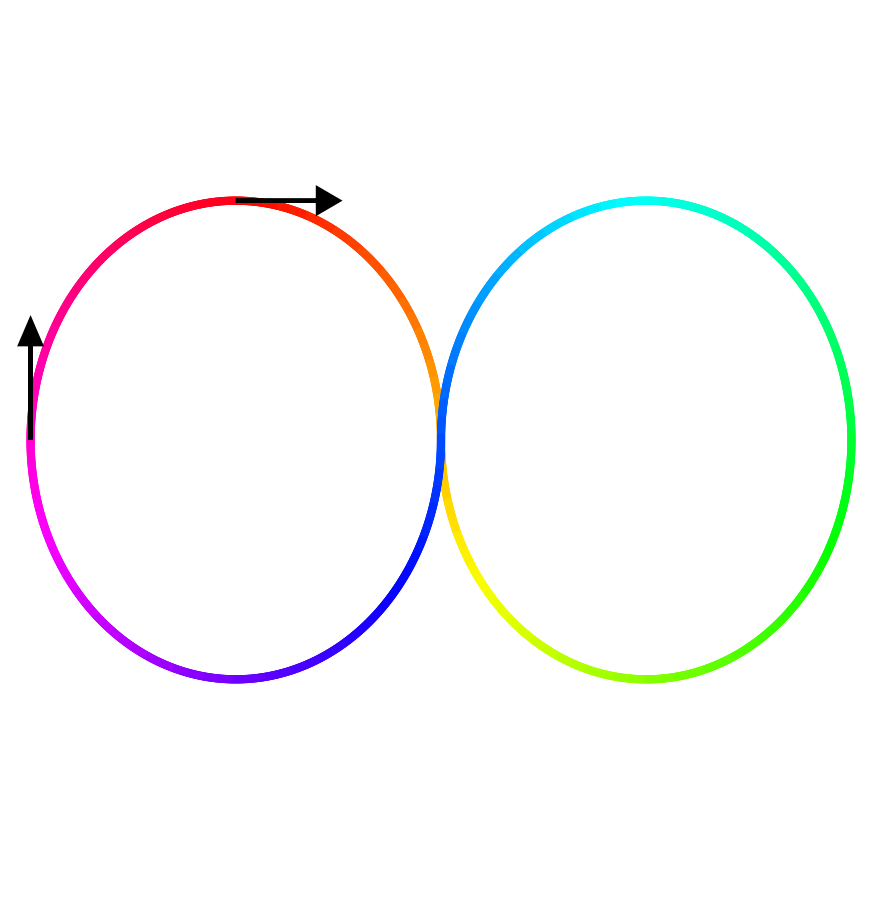
\includegraphics[width=.45\textwidth]{cmp3/tr2.png}
	}
	\subfigure[Embedding with a CNN AE.]{
		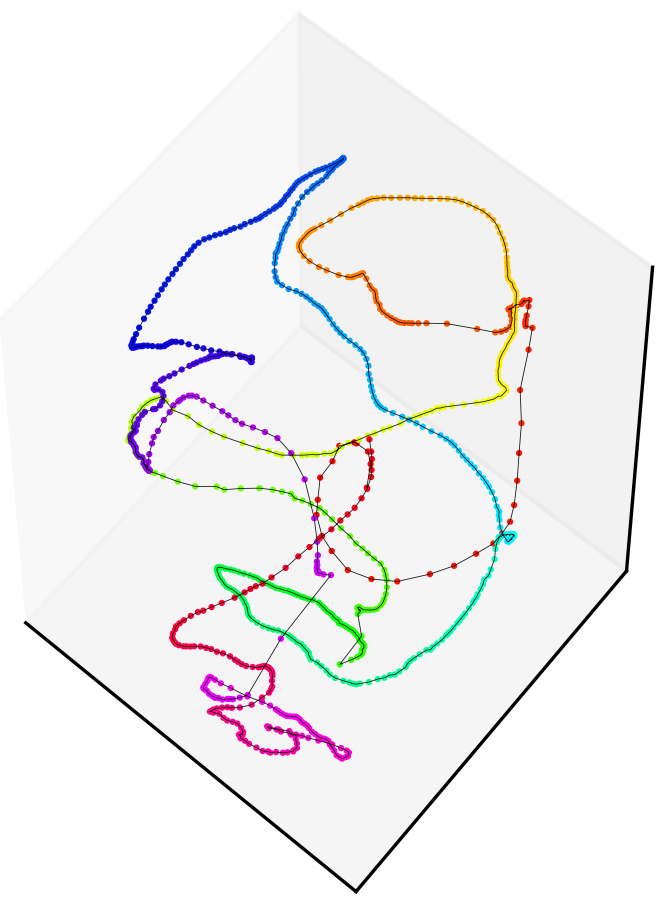
\includegraphics[width=.45\textwidth]{cmp3/cnn4_2.png}
	}\\
  \subfigure[Frames from the \textit{Eight} self-intersection trajectory.]{
    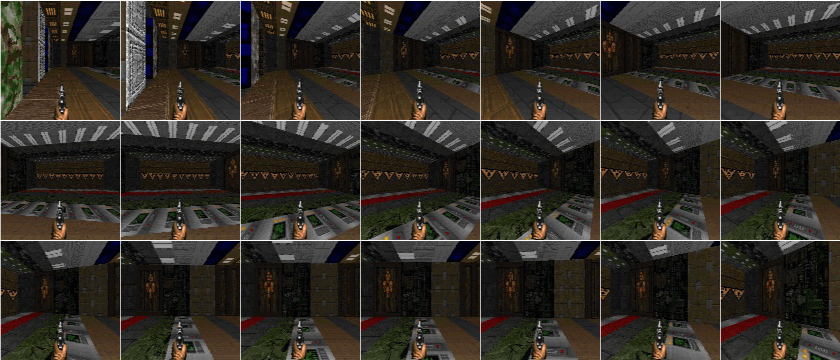
\includegraphics[width=.90\textwidth]{sprite2.png}
  }\\
    	\caption{Embedding a closed self-intersecting trajectory $(a, c)$ in a lower dimensional space using CNN AE. Black arrows on the reference trajectory indicate the direction of the player's view. Each embedding frame is visualized as time-colored point, subsequent frames are connected by a black line.}
    	\label{fig:model_param}
\end{figure}

Our experiments revealed, that models, based on a fully connected configuration show either similar or worth results comparing to CNN for more complex datasets while following the same trends as below. We therefore only provide results for better performing convolutional models.

We tested our training method on 8 possible configurations of the regularization. Best values of the error weight were selected with a grid search and has been fixed throughout the training. Model without any regularization showed
no improvement according to the predictive metric and binary predictive metric is well below 50\%. Yet, model was able to preserve 61.7\% of nearest neighbor relations.

When using a single type of regularization all 3 methods showed comparable results. Using a single regularization allows 5 to 8\% more accurate prediction of the next position on the manifold. Prediction of the future frame was more accurate than naive prediction in around 61-65\% of the time. In terms of reconstruction quality predictive regularization allowed to archive significant improvement over the non-regularized model. Interestingly, applied alone, denoising regularization showed the best results among the 3.

Among 3 models utilizing 2 types of regularization all showed at least marginal improvement over models with single regularization technique with "Predictive and distance" regularized model sharply outperforming all the others. "Predictive and distance" showed 59\% improvement in accuracy of future position prediction with 91\% of predictions being more accurate than naive prediction. It also managed to maintain 91\% of nearest neighbor relations in the embedding space.Reconstruction accuracy decreased.

Adding Denoising regularization to the best model so far did not have any significant effect as shown in the last line of the table \ref{tab:8emb}. We therefore take the combination of predictive and distance regularization as the main configuration of the model.


\subsection{Dataset complexity}

In this section we test our low-dimensionality embedding method on a large realistic dataset. We further evaluate test model on a trajectory which is not present in the training set, although recorded on the same map. We use a long continuous trajectory on a single \texttt{Doom II} map containing 300000 training images.
As validation we use a "circle" and an "eight" continuous trajectory similar to one described in previous experiment.
Data collection method guaranties, that while train and validation trajectories might contain similar or identical images, this images do not appear in duplicated subsequences i.e. if $t_i = v_j$ than $t_{i+1} \neq v_{j+1}$ for $\forall i \leq |T|$, where $T, V$ are validation and training sets. This constrain allows us to state, that even if continuity of training trajectory is imposed explicitly by the predictive regularization and only indicates overfitting, validation data shall not have the same quality.

\begin{table}
\begin{center}
    \begin{tabular}{| l | l | l | l | l |}
      \hline
     Model configuration  &  $P_{L2}$ & $P_{\beta}$ & $P_{\tau}$ & $L_{reco}$ \\ \hline
     16c3-p2-32c3-p2-32c3-p2-16c3-f3     & 0.000 & 0.222 & 0.356 & 69.98 \\
     16c3-p2-32c3-p2-32c3-p2-16c3-f100-f3 & 0.000 & 0.246 & 0.376 & 66.72 \\
     16c3-p2-32c3-p2-32c3-p2-16c3-f250-f3 & 0.000 & 0.249 & 0.387 & 66.72 \\
     16c3-p2-32c3-p2-32c3-p2-16c3-f250-f4 & 0.000 & 0.225 & 0.474 & 65.08 \\
     16c3-p2-32c3-p2-32c3-p2-16c3-f8      & 0.000 & 0.091 & 0.588 & 64.30 \\
     16c3-p2-32c3-p2-32c3-p2-16c3-f80-f8  & 0.000 & 0.149 & 0.587 & 57.09 \\ \hline
     \end{tabular}
\end{center}
  \caption{Validation performance of different model configurations on a large training set with multiple degrees of freedom.}
  \label{tab:large}
\end{table}

\begin{figure}[t!]
	\centering
	\subfigure[Trivial \textit{eight} trajectory as on figure \ref{fig:model_reco}(a) ]{
  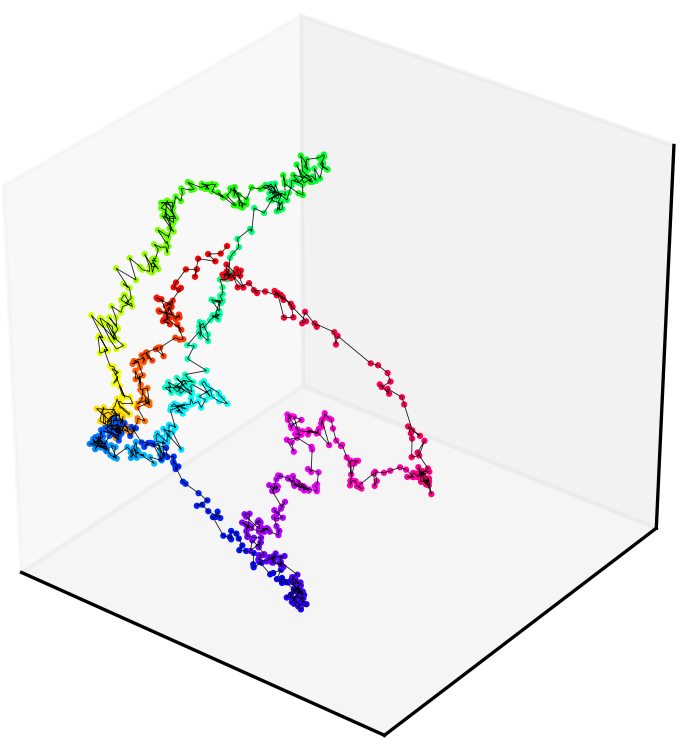
\includegraphics[width=.45\textwidth]{cmp4/cnn8.png}
	}
	\subfigure[Closed self-intersecting trajectory as on figure \ref{fig:model_param}(a)]{
		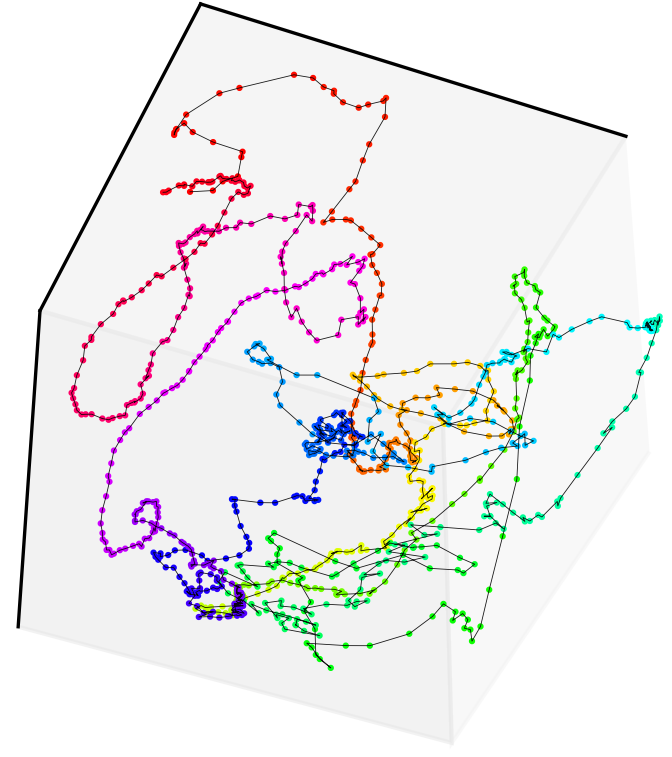
\includegraphics[width=.45\textwidth]{cmp4/cnn82.png}
	}\\
    	\caption{Visualization of first 3 components of 8 dimensional embedding of a validation closed self-intersecting trajectories. Projection is learned by a mixed CNN-FC AE model with next configuration: 16c3-p2-32c3-p2-32c3-p2-16c3-f80-f8.}
    	\label{fig:model_big}
\end{figure}

In this experiment we explored several higher complexity models using different dimensionality of the embedding space: 3, 4 or 8 components. We also experimented with a mixed CNN-FC model, allowing the final layers of the projection (encoder) network to have more complex projection form. We simplicity, we provide a short description of the network architecture in the table \ref{tab:large}. We use next notation to describe network architecture of the encoder: \textit{16c3-p2-32c3-p2-32c3-p2-16c3-f100-f3}. Where first \textit{16c3} corresponds to the first network layer.  \textit{16c3} indicates that layer has 16 convolutional filters of size $3 \times 3$. It is followed by a max-pooling layer $p2$ with stride equal 2. Final layers of the encoder are two fully connected layers  \textit{f100-f3} with 100 and 3 neurons correspondingly. Convolutional layers rely on the ReLU activation function while fully connected layers use logistic sigmoid, as described in section \ref{ss:cnnaec}.

Visual inspection of the embedding even without using dimensionality reduction techniques, showed that trajectory prototype maintains the characteristics actual players path. Namely it intersects itself only in a single place and the time of intersection corresponds to the time of the actual intersection of the trajectory. Yet, the path prototype appear entangled and relatively noisy comparing to previous experiments.

While embedding of the validation trajectory showed continuous form and maintained key intersection, actual model scores are quite low. None of the models was able to provide any improvement in terms of the prediction of the next frame, indicating highly non-linear manifold space at current level of input video discretization.

Models with higher dimensional embedding space showed better performance in terms of maintaining nearest neighbor relation in the embedding space: up to 58\% of $P_{\tau}$ score. They also allowed resulted in reconstruction of the input images. At the same time, predictive score of these models dropped.

Adding another fully connected layer before the last layer of the encoder led to the marginal improvement of all metrics and, more noticeably, of the reconstruction error. Yet, we don't see adding another highly parameterized layer in such a was as a significant advantage.


\subsection{Relevance of the depth information}

In this section we compare effects of the presence or absence of the depth information in the training data. Most of the first person video data comes in form of RGB video channel, that does not contain information about the distance to the objects. In this section we try to asses, how relevant is this information to the task at hand. Results of the experiments for trivial trajectory (see \ref{fig:model_reco}(a)) and an \textit{eight} trajectory (see \ref{fig:model_param}(a)) are shown below.

\begin{table}
\begin{center}
    \begin{tabular}{| l | l | l | l | l |}
      \hline
     Model configuration  &  $P_{L2}$ & $P_{\beta}$ & $P_{\tau}$ & $L_{recoRGB}$ \\ \hline
     Trivial trajectory without depth info		& 0.135 & 0.498 & 0.676 & 63.87 \\
     Trivial trajectory with depth info 		& 0.178 & 0.509 & 0.699 & 64.86 \\ \hline
     "Eight" trajectory without distance information	 	& 0 & 0 & 0 & 86.60 \\
     "Eight" trajectory with distance information		   & 0.476 & 0.778 & 0.236 & 75.49 \\ \hline
    \end{tabular}
\end{center}
  \caption{Comparison of model performance on 2 distinct trajectories depending on presence or absence of the depth information. $L_{recoRGB}$ is calculated only for RGB channels for all models.}
  \label{tab:depth}
\end{table}

Results show, that presence of the depth information in the training data is crucial for the learning the task at hand. Namely, in case of the trivial self-intersecting trajectory depth channel allowed to improve all 3 scores at hand at a low cost of reconstruction error, which is irrelevant to the task at hand. In case of a more complex trajectory model was not able to learn the concept at all without the depth information and projected all points of the trajectory into a single point on the manifold.

% !TEX root = ./thesis.tex

\chapter{Discussion}
\label{ch:conc}

In this work we proposed a deep-learning technique for mapping sequences of visual data into a manifold space while preserving key spatial relations. We analyzed the effectiveness of our approach on tasks of varying complexity. Experiments showed, that model is capable to learn effectively some trivial trajectories and reveal some structure in more complex cases. Learned solutions typically reveal local spatial relation in the data and allow to identify self-intersecting trajectories. We showed, that even while working with exclusively visual data, out approach allows to create approximate prediction of the future position and possible visual frames.    


\listoffigures
\listoftables

%%%----------------------------------------------------------
%%%Anhang
\appendix
% \include{anhang_a}	% Technische Ergänzungen
% \include{anhang_b}	% Inhalt der CD-ROM/DVD
% \include{anhang_c}	% Chronologische Liste der Änderungen
% \include{anhang_d}	% Quelltext dieses Dokuments

%%%----------------------------------------------------------
\MakeBibliography
%%%----------------------------------------------------------

%%%Messbox zur Druckkontrolle
\include{messbox}

\end{document}
